%% 
%% Copyright 2007-2020 Elsevier Ltd
%% 
%% This file is part of the 'Elsarticle Bundle'.
%% ---------------------------------------------
%% 
%% It may be distributed under the conditions of the LaTeX Project Public
%% License, either version 1.2 of this license or (at your option) any
%% later version.  The latest version of this license is in
%%    http://www.latex-project.org/lppl.txt
%% and version 1.2 or later is part of all distributions of LaTeX
%% version 1999/12/01 or later.
%% 
%% The list of all files belonging to the 'Elsarticle Bundle' is
%% given in the file `manifest.txt'.
%% 

%% Template article for Elsevier's document class `elsarticle'
%% with numbered style bibliographic references
%% SP 2008/03/01
%%
%% 
%%
%% $Id: elsarticle-template-num.tex 190 2020-11-23 11:12:32Z rishi $
%%
%%
% \documentclass[preprint,12pt]{elsarticle}

%% Use the option review to obtain double line spacing
% \documentclass[authoryear,preprint,review,12pt]{elsarticle}

%% Use the options 1p,twocolumn; 3p; 3p,twocolumn; 5p; or 5p,twocolumn
%% for a journal layout:
%% \documentclass[final,1p,times]{elsarticle}
\documentclass[5p,times]{elsarticle}
%% \documentclass[final,3p,times]{elsarticle}
%% \documentclass[final,3p,times,twocolumn]{elsarticle}
%% \documentclass[final,5p,times]{elsarticle}
%% \documentclass[final,5p,times,twocolumn]{elsarticle}

%% For including figures, graphicx.sty has been loaded in
%% elsarticle.cls. If you prefer to use the old commands
%% please give \usepackage{epsfig}
\usepackage[table, dvipsnames]{xcolor}

\definecolor{Mycolor1}{HTML}{4C5866} %#4C5866
\definecolor{Mycolor2}{HTML}{A6B6D2} %#A6B6D2
\definecolor{Mycolor3}{HTML}{67daff} %#67daff
\definecolor{Mycolor4}{HTML}{F7F7FE} %#F7F7FE
\definecolor{Mycolor5}{HTML}{666ad1} %#666ad1
\definecolor{Mycolor6}{HTML}{ffbb93} %#ffbb93
\newcommand{\mycolorbox}[2]{\begingroup\setlength{\fboxsep}{2pt}\colorbox{#1}{#2}\endgroup}

% cite with author names
\newcommand{\citea}[1]{\citeauthor{#1}~\cite{#1}}
\newcommand{\bobgraph}[1]{\noindent\textbf{#1}}

% draw a colored square
% color, width, height
\newcommand\coloredsquare[3][black]{\textcolor{#1}{\rule{#2}{#3}}} 

% thumbnail image
\usepackage{wrapfig}
\newcommand{\thumbnail}[2]{
    \begin{samepage}

      \setlength{\intextsep}{3pt}
      \setlength{\columnsep}{3pt}
      \begin{wrapfigure}{r}{0.4\columnwidth}
        \vspace{-15pt}
        \begin{center}
          \includegraphics[width=0.35\columnwidth]{"#1".png}
        \end{center}
      \end{wrapfigure}
      #2
      
    \end{samepage}
}


% list with styles
\usepackage{enumitem}

%% The amssymb package provides various useful mathematical symbols
\usepackage{amsmath,bm}
\usepackage{amssymb}
%% The amsthm package provides extended theorem environments
%% \usepackage{amsthm}

%% The lineno packages adds line numbers. Start line numbering with
%% \begin{linenumbers}, end it with \end{linenumbers}. Or switch it on
%% for the whole article with \linenumbers.
%% \usepackage{lineno}

\usepackage{float,hhline,array,tabulary,tabularx,etoolbox,multirow,multicol}

\usepackage{moreverb,url}

\newcommand{\algorithmautorefname}{Algorithm}
\usepackage{algpseudocode}
\usepackage{algorithm}
% switch for algorithmic
% New definitions
\algnewcommand\algorithmicswitch{\textbf{switch}}
\algnewcommand\algorithmiccase{\textbf{case}}
\algnewcommand\algorithmicdefault{\textbf{default}}

\algdef{SE}[SWITCH]{Switch}{EndSwitch}[1]{\algorithmicswitch\ #1\textbf{:}}{\algorithmicend\ \algorithmicswitch}%
\algtext*{EndSwitch}%

\algdef{SE}[CASE]{Case}{EndCase}[1]{\algorithmiccase\ #1\textbf{:}}{\algorithmicend\ \algorithmiccase}%
\algtext*{EndCase}%

\algdef{SE}[DEFUALT]{Default}{EndDefault}{\algorithmicdefault\textbf{:}}{\algorithmicend\ \algorithmicdefault}%
\algtext*{EndDefault}%

\algnewcommand\algorithmicforeach{\textbf{for each}}
\algdef{S}[FOR]{ForEach}[1]{\algorithmicforeach\ #1\ \algorithmicdo}

% code listing
\usepackage{listings}
\lstdefinestyle{customc}{
  belowcaptionskip=1\baselineskip,
  breaklines=true,
  xleftmargin=\parindent,
  language=C,
  showstringspaces=false,
  basicstyle=\footnotesize\ttfamily,
  keywordstyle=\bfseries\color{green!40!black},
  commentstyle=\itshape\color{purple!40!black},
  identifierstyle=\color{blue},
  stringstyle=\color{orange},
}

\lstdefinestyle{customasm}{
  belowcaptionskip=1\baselineskip,
  xleftmargin=\parindent,
  language=[x86masm]Assembler,
  basicstyle=\footnotesize\ttfamily,
  commentstyle=\itshape\color{purple!40!black},
}

\lstset{escapechar=@,style=customc}

% bold \mathcal{}
\DeclareMathAlphabet{\mathbcal}{OMS}{cmsy}{b}{n}

% wrapper for math symbols
\newcommand{\Vector}[1]{\protect\overrightarrow{#1}}
\newcommand{\Line}[1]{\protect\overline{#1}}
\newcommand{\dx}{\Delta x}
\newcommand{\dy}{\Delta y}
\newcommand{\Width}[1]{\lvert #1 \rvert}

% UpdateNodePosition
\newcommand{\nodeList}{\bm{L}}

\newcommand{\nodeFNORLine}{\Line{\node\nodeFNOR}}
\newcommand{\nodeSize}{s}
\newcommand{\nodeSizeAvg}{\nodeSize_{avg}}
\newcommand{\nodeSizeMax}{\nodeSize_{max}}
\newcommand{\nodeError}{\epsilon}
\newcommand{\nodeCartographicError}{\nodeError_{c}}
\newcommand{\nodeCartographicErrorMax}{\nodeError_{c_{max}}}
\newcommand{\nodeTopologicalError}{\nodeError_{t}}
\newcommand{\nodeTopologicalErrorMax}{\nodeError_{t_{max}}}
\newcommand{\stalemateMax}{w}
\newcommand{\nodeCross}{\node.cross}
\newcommand{\nodeListCross}{\nodeList.cross}
\newcommand{\nodeListCrossCount}{\nodeList.count}

% move position

\newcommand{\node}{\bm{n}}
\newcommand{\nodePrevious}{\node_{p}}
\newcommand{\nodeFNOR}{\node_t}

\newcommand{\nodeVectorTC}{\Vector{\nodeFNOR\node}}
\newcommand{\nodeVectorCT}{\Vector{\node\nodeFNOR}}

% check river crossing

\newcommand{\river}{\bm{r}}
\newcommand{\riverVector}{\Vector{v_{\river}}}
\newcommand{\riverList}{\bm{R}}
\newcommand{\nodeBoundingBox}{b_{\Line{n}}}
\newcommand{\riverEdgeBoundingBox}{b_{\Edge}}
\newcommand{\boundingBoxInt}{b_{int.}}
\newcommand{\nodeEdge}{e_n}
\newcommand{\edgeBoxInt}{e_{int.}}

% derive corridor
\newcommand{\Corridor}{c}
\newcommand{\CorridorLength}{\Corridor_l}
\newcommand{\CorridorWidth}{\Corridor_w}
\newcommand{\PointP}{\node_c}
\newcommand{\Edge}{\Line{e}}
\newcommand{\EdgeStart}{\Edge.start}
\newcommand{\EdgeEnd}{\Edge.end}
\newcommand{\EdgeParallel}{\Line{e_p}}
\newcommand{\EdgeParallelA}{\Line{e_{p^1}}}
\newcommand{\EdgeParallelB}{\Line{e_{p^2}}}
\newcommand{\Distance}{d}
\newcommand{\nodeVectorNP}{\Vector{\node\PointP}}
\newcommand{\nodeVectorNV}{\Vector{\node\nodeFNOR}}
\newcommand{\nodeLineNV}{\Line{\node\nodeFNOR}}
\newcommand{\nodeLinePN}{\Line{\nodePrevious\node}}
\newcommand{\nodeVectorNtP}{\Vector{\nodeFNOR\PointP}}
\newcommand{\nodeLineNtNc}{\Line{\nodeFNOR\PointP}}
\newcommand{\nodeLineWidthNtP}{\Width{\nodeFNOR\PointP}}
\newcommand{\nodeInCorridor}{\node_{in}}
\newcommand{\nodeInCorridorT}{\node_{in_t}}


% derive corridor point
\newcommand{\Scale}{scale}

% figure fig:corridor

\newcommand{\nodeVectorNNn}{\Vector{\node\node_{t}}}
\newcommand{\nodeVectorNinNinn}{\Vector{\nodeInCorridor\nodeInCorridorT}}


\newcommand{\vectorAvg}{\bm{v}_{avg}}
\newcommand{\NxR}{\node_{n_{x}r}}
\newcommand{\RxN}{\node_{r_{x}n}}

\usepackage[nameinlink]{cleveref}

\newcommand\BibTeX{{\rmfamily B\kern-.05em \textsc{i\kern-.025em b}\kern-.08em
T\kern-.1667em\lower.7ex\hbox{E}\kern-.125emX}}


% \journal{Nuclear Physics B}

\begin{document}

\begin{frontmatter}

    %% Title, authors and addresses

    %% use the tnoteref command within \title for footnotes;
    %% use the tnotetext command for theassociated footnote;
    %% use the fnref command within \author or \address for footnotes;
    %% use the fntext command for theassociated footnote;
    %% use the corref command within \author for corresponding author footnotes;
    %% use the cortext command for theassociated footnote;
    %% use the ead command for the email address,
    %% and the form \ead[url] for the home page:
   
    \title{Demers Cartogram with Rivers}

    \begin{abstract}
        Cartograms serve as representations of geographical and abstract data, employing a value-by-area mapping technique.
        As a variant of the Dorling cartogram, the Demers cartogram utilizes squares instead of circles to represent regions.
        This alternative approach allows for a more intuitive comparison of regions, utilizing screen space more efficiently.
        However, a drawback of the Dorling cartogram and its variants lies in the potential displacement of regions from their original positions, ultimately compromising legibility, readability, and accuracy.
        To tackle this limitation, we propose a novel hybrid cartogram layout algorithm that incorporates topological elements, such as rivers, into Demers cartograms.
        The presence of rivers significantly impacts both the layout and visual appearance of the cartograms.
        Through a user study conducted on an Electronic Health Records (EHR) dataset, we evaluate the efficacy of the proposed hybrid layout algorithm.
        The obtained results illustrate that this approach successfully retains key aspects of the original cartogram while enhancing legibility, readability, and overall accuracy.

    \end{abstract}

    \begin{keyword}
        Cartogram \sep Demers Cartogram \sep Visual Analytics \sep EHR Visualization

    \end{keyword}

\end{frontmatter}

%% \linenumbers

%% main text
\section{Introduction and Motivation}
\label{}
Cartograms are representations of geographical and abstract data based on a value-by-area mapping combining statistical and geographical information \cite{dent2009Cartography,inoue2011New}.
Various styles of cartograms have been proposed and implemented for applications such as urban planning \cite{harris2018Mapping, arranz-lopez2021Enduser}, natural hazard forecasting \cite{pappenberger2019Cartograms, park2020Flood}, conservation and environmental planning \cite{galluzzi2018Mapping, rocchini2019Cartogramming}, political and social demographics \cite{breitzman2018Using, alieva2021How}, and decision-making for public health \cite{gao2020Visualising, sack2021Visualizing}.

\begin{figure}[htpb]
    \centering
    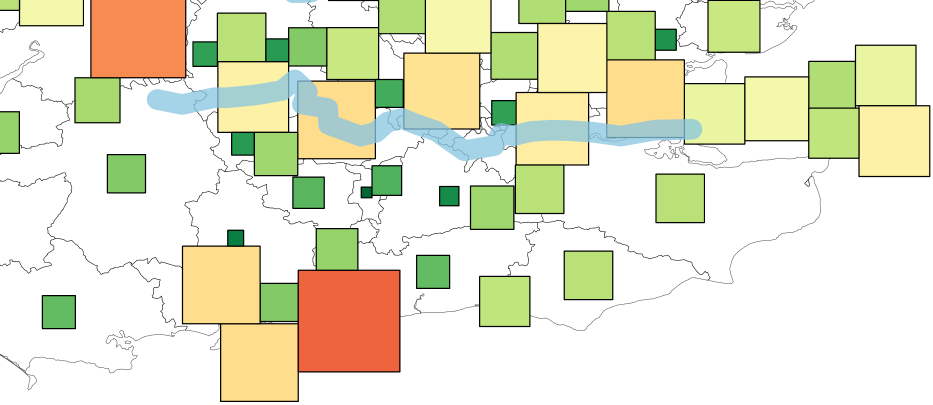
\includegraphics[width=0.8\linewidth,keepaspectratio]{cover.png}
    \caption{The River Thames passing through a cartographic representation of the NHS CCGs in London and surrounding areas.}
    \label{fig:cover}
\end{figure}

Among the four types of cartogram categorized in a survey by \citet{nusrat2016State} (See \Cref{sec:RelatedWork} for definitions of contiguous, non-contiguous, rectangular, and Dorling), a trade-off is made between types of accuracy (See \Cref{table:accuracy}).
For this project, we focus on non-contiguous cartograms like Demers cartograms because they facilitate statistical comparison between regions, they can make good use of screen space, and comparison of regions is useful when studying Electronic Health Records (EHR) data.
Demers cartograms offer the advantage in cases where the data is not directly correlated to region sizes.
In other words, Demers cartograms are useful when a data dimension is not describing the geography of the region it represents but is tied to something else, for example the health of its population.
Also, the comparison of magnitudes becomes an area estimation task, which is effective for a numeric data encoding \cite{munzner2014Visualization}.
See \citea{nickel2022Multicriteria} for a more complete description of the advantages that Demers cartograms offer.
Building on Demers cartograms \cite{ian2002Cartogram}, we introduce and develop novel features, such as rivers, aiming to improve the readability and geographical accuracy without sacrificing statistical accuracy.
Standard Demers cartograms are composed of square nodes that representing geographic enumeration units.
As such, this can reduce their legibility.
We implement a new hybrid cartographic layout algorithm that combines rivers with the placement of the nodes representing geographic enumeration units, in this case, a Clinical Commissioning Group (CCG).
We hypothesize that introducing rivers improves the overall legibility of a cartogram.
By \textit{legibility} we mean readability and ability to interpret the cartogram.
To assess this hypothesis, we designed an experimental setup where participants engaged in correspondence and location tasks as part of a user study.
To reduce error and make efficient use of screen space, the algorithm also updates the position of rivers to accommodate the node layout.
We then apply the algorithm to a real-world case study using EHR data to evaluate the result.
We present a user study that demonstrates its effectiveness.

Our contributions include:

\begin{itemize}
    \setlength\itemsep{0px}
    \item A new variant of Demers cartograms that incorporates rivers to improve readability and recognizability,
    \item A novel hybrid layout algorithm that combines node positions with features such as rivers,
    \item A user study evaluation of the technique with an application to EHRs.
\end{itemize}

The results of the user study indicate that rivers can improve the legibility of cartograms.
One of the major challenges involved is developing a layout algorithm that handles different shapes.
In other words, the hybrid layout algorithm is novel because it handles different types of elements: square node representing regions and polylines representing rivers.
Another challenge we overcome in developing the algorithm is to resolve stalemate situations where nodes become congested due to constraints imposed by rivers, while ensuring error minimization.


\section{Related Work}
\label{sec:RelatedWork}

This section introduces the characteristics of various cartogram styles, describes relevant applications of cartograms, and provides a brief overview of some real-world implementations of cartogram-based visualizations.

\subsection{Definitions}

While we focus on rectangular cartogram variants, we start with brief definitions of contiguous and non-contiguous cartograms: Contiguous cartograms preserve topology, maintain connectivity with their adjacent neighbors, but are also subject to distortion in shape.
Non-contiguous cartograms sacrifice topological connectivity with neighbors to enable expansion or reduction in size while maintaining their polygonal shape \cite{dent2009Cartography}.

\citet{nusrat2016State} define and summarize three major accuracy dimensions for cartograms: statistical, geographical, and topological.
Each cartogram design may make various types of accuracy trade-offs between dimensions.
We provide a comparison of these trade-offs as introduced by \citet{nusrat2016State} in \Cref{table:accuracy}.
In addition, we include the Demers as it is the focus of our work.

    {
        \renewcommand{\arraystretch}{1.5}
        \begin{table*}[!tb]
            \centering
            \resizebox{\textwidth}{!}{
                \begin{tabulary}{\textwidth}{|*{4}{l|}r|c|}
                    \hhline{~|*{4}{-}|~}
                    \multicolumn{1}{c|}{\textbf{Literature}} &
                    \textbf{Cartogram Type(s)} &
                    \textbf{Geographic Region(s)} &
                    \textbf{Number of Nodes} &
                    \multicolumn{1}{c|}{\textbf{Year}} \\
                    \hline

                    % \citet{auber2007Geographical} & \citep{auber2007Geographical} & US & 19 & 2007 \\
                    % \hline
                    \citet{warf2008Geography} & Dorling & US & 3,142 & \citeyear{warf2008Geography} \\
                    \hline
                    \citet{sun2010Effectiveness} & Dorling, Mosaic, Neighbor-preserving & US, China & 34 - 49 & \citeyear{sun2010Effectiveness} \\
                    \hline
                    \citet{cruz2017Adapted} & Dorling, Non-contiguous, Neighbor-preserving & Portugal & 2,882 & \citeyear{cruz2017Adapted} \\
                    \hline
                    \citet{tong2018Cartograms} & Demers & England & 209 & \citeyear{tong2018Cartograms} \\
                    \hline
                    \citet{gao2020Visualising} & Dorling & China & 34 & \citeyear{gao2020Visualising} \\
                    \hline
                    \citet{nusrat2020Recognition} & Contiguous, Dorling & US & 49 & \citeyear{nusrat2020Recognition} \\
                    \hline
                    \citet{nickel2022Multicriteria} & Non-contiguous, Demers & US, Netherlands, World & 49 - 342 & \citeyear{nickel2022Multicriteria} \\
                    \hline

                    % \multicolumn{1}{c|}{\textbf{Total unique papers: 51}} & 24&15&12& \multicolumn{1}{c}{}  \\
                    % \hhline{~|*{3}{-}|~}

                \end{tabulary}
            }
            \caption{Related work with non-contiguous cartogram-based visualizations.
                \textbf{Cartogram type} is the type of cartogram used.
                \textbf{Geographic region} is the geographic region depicted by the cartogram.
                \textbf{Number of nodes} is the number of nodes (representing geographic enumeration units) depicted in the cartogram.
            }
            \label{table:region vs node}
        \end{table*}
    }

\thumbnail{dorling}{
    \bobgraph{Dorling cartograms}, as a variant of non-contiguous cartograms, generally do not preserve geography and topology.
    A Dorling cartogram is statistically accurate, regions are represented by circles and the data dimensions of interest are represented by the circle area \cite{dorling2011Area}.
    In a Demers cartogram, a variant of Dorling, squares are used instead to capture a certain level of topology, as described by \citet{cano2015Mosaic} in their related work section.
    Dorling cartograms are unable to maintain topological accuracy as circles are often repositioned to remove overlap.
    Here we focus on Demers cartograms as we use squares to depict regions.
    This style of cartogram offers the advantages that the comparisons between regions are intuitive and screen space utilization is more efficient.
    This is important in our use case scenario involving EHRs.
    Demers cartograms, where regions are represented by squares, often have the advantage of preserving a higher level of topology at the cost of geographical accuracy \cite{ian2002Cartogram}.
}

\thumbnail{rectangular}{
    \bobgraph{Rectangular cartograms} are contiguous and do not preserve geographical accuracy \cite{raisz1934Rectangular, vankreveld2004Rectangular}.
    Depending on the variant, a rectangular cartogram may trade-off between statistical and topological accuracy.
}

\thumbnail{mosaic}{
    \bobgraph{Mosaic cartograms} usually use square or hexagonal tiles to depict regions, and are contiguous and sacrifice statistical accuracy to preserve some level of geographical accuracy \cite{cano2015Mosaic}.
    Some variants are able to preserve topological accuracy as well.
}

{
    \renewcommand{\arraystretch}{1.5}
    \begin{table}[!tb]
        \centering
        \resizebox{\columnwidth}{!}{
            \begin{tabulary}{\columnwidth}{|*{5}{l|}}
                \hhline{~|*{3}{-}|~}
                \multicolumn{1}{c|}{} & \multicolumn{3}{c|}{\cellcolor{Mycolor2} \textbf{Accuracy}} \\
                \hhline{~|*{4}{-}}
                \multicolumn{1}{c|}{\textbf{Cartogram Variant}} &
                \textbf{Statistical} &
                \textbf{Geographical} &
                \textbf{Topological} &
                \textbf{Contiguity} \\
                \hline
                Contiguous & \cellcolor{Mycolor3}Variable & \cellcolor{Mycolor3}Variable & Accurate & Yes \\
                \hline
                Non-contiguous & \cellcolor{Mycolor5}\textcolor{white}{Accurate} & \cellcolor{Mycolor5}\textcolor{white}{Shape is accurate} &\cellcolor{Mycolor6}Inaccurate & No   \\
                \hline
                Rectangular & \cellcolor{Mycolor3}Variable & Shape is inaccurate & \cellcolor{Mycolor3}Variable & Yes   \\
                \hline
                Dorling & Accurate & \cellcolor{Mycolor6}Inaccurate & \cellcolor{Mycolor3}Variable & No  \\
                \hline
                Demers & Accurate & \cellcolor{Mycolor6}Inaccurate & \cellcolor{Mycolor3}Variable & No  \\
                \hline
            \end{tabulary}
        }
        \caption{\coloredsquare[Mycolor3]{0.25cm}{0.25cm} Trade-off between dimensions.
            \coloredsquare[Mycolor6]{0.25cm}{0.25cm} Dimension sacrificed in order to improve \coloredsquare[Mycolor5]{0.25cm}{0.25cm} target dimension's accuracy.}
        \label{table:accuracy}
    \end{table}
}

\subsection{Peer-reviewed Applications}

There has been a substantial amount of research done in this area, here we review some of the important work that has inspired our work.\citet{warf2008Geography} use a Dorling cartogram to represent religious diversity in the US.
\citet{sun2010Effectiveness} depict 1996 US election data and 2005 Chinese population data using Dorling, Mosaic, and contiguous cartograms.
\citet{gao2020Visualising} present a Dorling cartogram to illustrate COVID-19 infections in China.
\citet{tong2018Cartograms} use a Demers cartogram to visualize health-related data by CCG regions in England, the work introduces a novel technique to remove the overlap of squares based on topological features, aiming to improve both geographical and topological accuracy.
\citet{nusrat2020Recognition} investigate the memorability of contiguous and Dorling cartograms using multiple data sets that include demographic, agriculture, and retail data in the US.
See \Cref{table:region vs node} for a list of literature that adopts cartograms for visualization with corresponding geographical regions and node counts.

Our work extends the algorithm described by \citet{tong2018Cartograms} which incorporates a static topological feature into Demers cartograms.
Our work enhances that of \citet{tong2018Cartograms} in multiple ways.
First, we introduce multiple features (rivers) into the layout, as opposed to a single river.
Second, we make topological features dynamic and further improve legibility and geographical accuracy.
By the term \textit{dynamic}, we mean that the position of the rivers is updated as part of the layout algorithm.
In previous work, the river is static and serves merely as a boundary.
Third, we improve the algorithm to resolve stalemates.
Finally, the way we evaluate the cartograms is also different.
\citet{tong2018Cartograms} count river crossings to evaluate error (a statistical metric).
Here our focus is on readability, and thus we include a user study.

\subsection{Cartograms in Media}

Cartograms are an engaging visual representation and therefore they are a popular choice of representation in covering various topics by the media.
The Washington Post uses cartograms to visualize the US overseas economic assistance, in arm sales (Mosaic) \cite{bearak2016Everything}, the 2016 US Election (contiguous) \cite{gamio2016Election}, and the Brexit Referendum (Mosaic) \cite{taylor2016What}.
National Geographic uses contiguous and Mosaic cartograms to analyze the 2016 US Election results \cite{miller2016Election}, the same topic is also covered by the Financial Times with a Dorling cartogram \cite{stabe2016Search}.
\citet{cruz2017Adapted} adapts a Dorling cartogram with both contiguous and non-contiguous cartograms to represent the gender pay gap in Portugal.
\citet{sandberg2018Cartogram} reports the 2018 US midterm Election with a Mosaic cartogram, the same approach is used to cover the 2020 US Election by the New York Times \cite{thelearningnetwork2020What} and Bloomberg \cite{mccartney20202020}.

One of the disadvantages of Dorling and Demers cartograms is legibility.
The layout algorithms may displace regions far from their original position and make the maps more difficult to interpret.
\citet{nickel2022Multicriteria} present a method to compute stable Demers cartograms with multiple constraints to maintain adjacencies with no overlapping nodes.

In this paper, we introduce a new type of topological feature, a river, as a constraint to compute the final layout, with the aim of improving the interpretation, readability, and accuracy of this class of cartograms.

\section{Data Description}

 {
  \begin{figure}[b!]
      \centering
      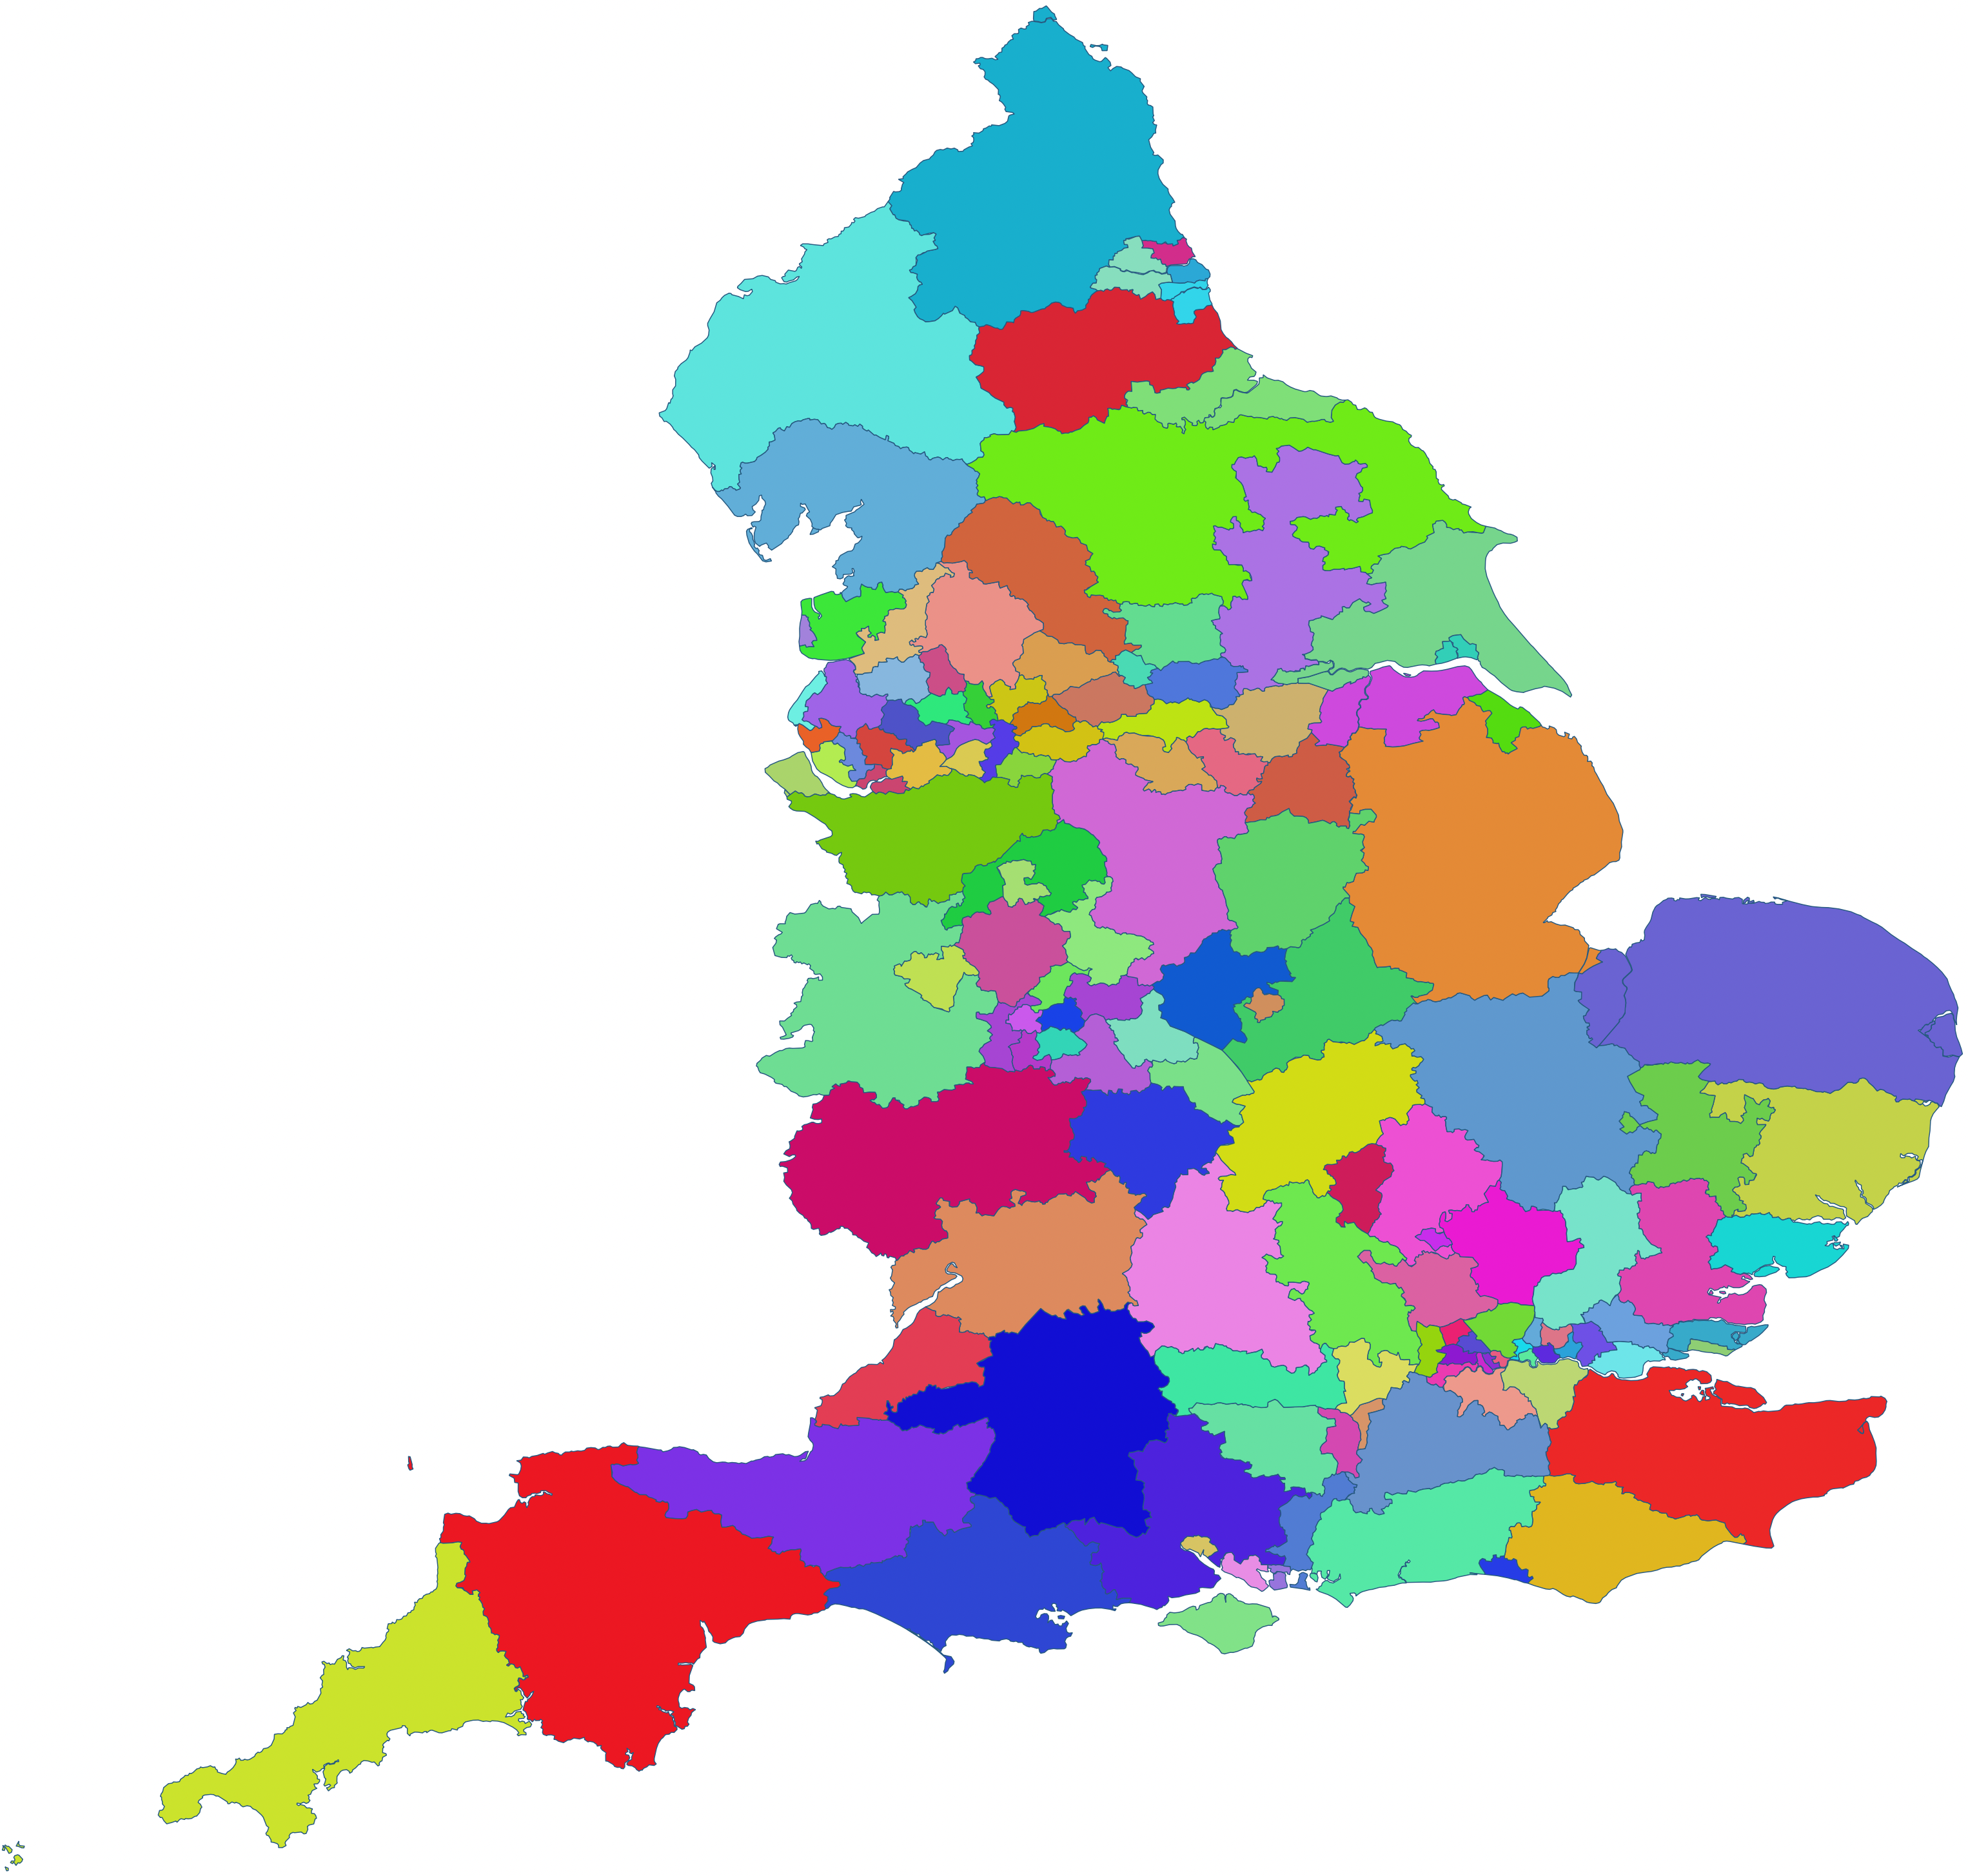
\includegraphics[width=0.6\columnwidth]{ccg.png}
      \caption{A map of 135 CCGs in England as of 2020, obtained from the Open Geography Portalx \cite{opengeographyportalxOpen} with EPSG:4326 (WGS84 - World Geodetic System) as the Coordinate Reference System (CRS).}
      \label{fig:ccg}
  \end{figure}
 }

Processing heterogeneous data can be challenging, especially when an EHR dataset is involved, because the data comes from multiple sources \cite{wang2021EHR}.
The first step is to obtain both geospatial boundaries and EHR data.
The second step is to preprocess the EHR data to remove empty and erroneous values.
The final step is to transform the data into a format that is suitable for cartograms.
Geospatial boundaries, or shapefiles, were obtained from the sources described here.

\subsection{Choropleth Shapefile}

Clinical Commissioning Groups (CCGs) are the primary administrative and geographic unit of the National Health Service (NHS) in the UK \cite{nhsNHS}.
The number of CCGs changes over time due to NHS reorganization.
The most up-to-date shapefile is available from the Open Geography Portalx \cite{opengeographyportalxOpen}.
We decided to use the CCG shapefile from 2020 at the time of writing, due to the absence of published public EHR data based on the latest CCG reorganizations that took place in 2021 and 2022.

\subsection{River Shapefiles}

We used OpenStreetMap \cite{openstreetmapRelation} as our data source to obtain shapefiles for the Thames River, the Trent River, and the Great Ouse River in England.
These rivers were chosen as they are well-known rivers, pass through regions with dense populations, and provide informative geographical and topological cues.
Although including smaller rivers is technically feasible, it may not increase the legibility of the cartogram.
This is an open question for future work.

We first obtain a relation ID by searching for a river, e.g.
River Thames, on OpenStreetMap.
The relation ID is used to construct a query (See \Cref{obtaining-shapefile}) which enables the user to download the entire river shapefile using Overpass Turbo \cite{overpassturboOverpass}.

After acquiring the shapefiles, we used QGIS \cite{qgisWelcome} to manually adjust the projections and convert them into GeoJSON files.
Finally, mapshaper \cite{blochMapshaper} is used to merge and convert the GeoJSON files into a TopoJSON file \cite{TopoJSON}.
TopoJSON eliminates redundant coordinates in the data, improving the rendering speed of our implementation.
See \Cref{table:pre-processing_result} on page \pageref{table:pre-processing_result} for the preprocessing result.
We describe the one-time preprocessing steps in more detail in \Cref{app:pre-processing}.

\subsection{EHR Data}

We obtained the Clinical Commissioning Group Outcomes Indicator Set (CCG OIS) from NHS Digital \cite{nhsdigitalClinical}.
The OIS is a set of indicators that are used to measure the quality of care and the associated health outcomes in the NHS.
Some datasets include:
\begin{itemize}
    \setlength\itemsep{0px}
    \item Under 75 mortality: cardiovascular disease, respiratory disease, liver disease, and cancer
    \item Emergency hospital admission: stroke, alcohol-specific admission and readmission, coronary heart disease, re-admissions within 30 days of discharge, children with lower respiratory tract infections
\end{itemize}

For all datasets, a spreadsheet including the following is provided:

\begin{itemize}
    \setlength\itemsep{0px}
    \item Reporting period: Calendar year of registration
    \item Period of coverage: Start and end date or reporting period
    \item Breakdown: Organization type
    \item ONS code: UK Office for National Statistics CCG code
    \item Level: CCG Code
    \item Level description: CCG Name
    \item Gender
    \item Indicator value: Directly standardized mortality rate
    \item CI lower: lower 95\% confidence interval
    \item CI upper: upper 95\% confidence interval
    \item Denominator: The count of registered patients
    \item Numerator: Number of deaths
\end{itemize}

Each CCG has a unique ONS code, which is used to link the CCG shapefile with the statistical data.

\section{Demers Cartogram with Rivers}
\label{sec:main}

{
    \begin{figure*}[tb!]
        \centering
        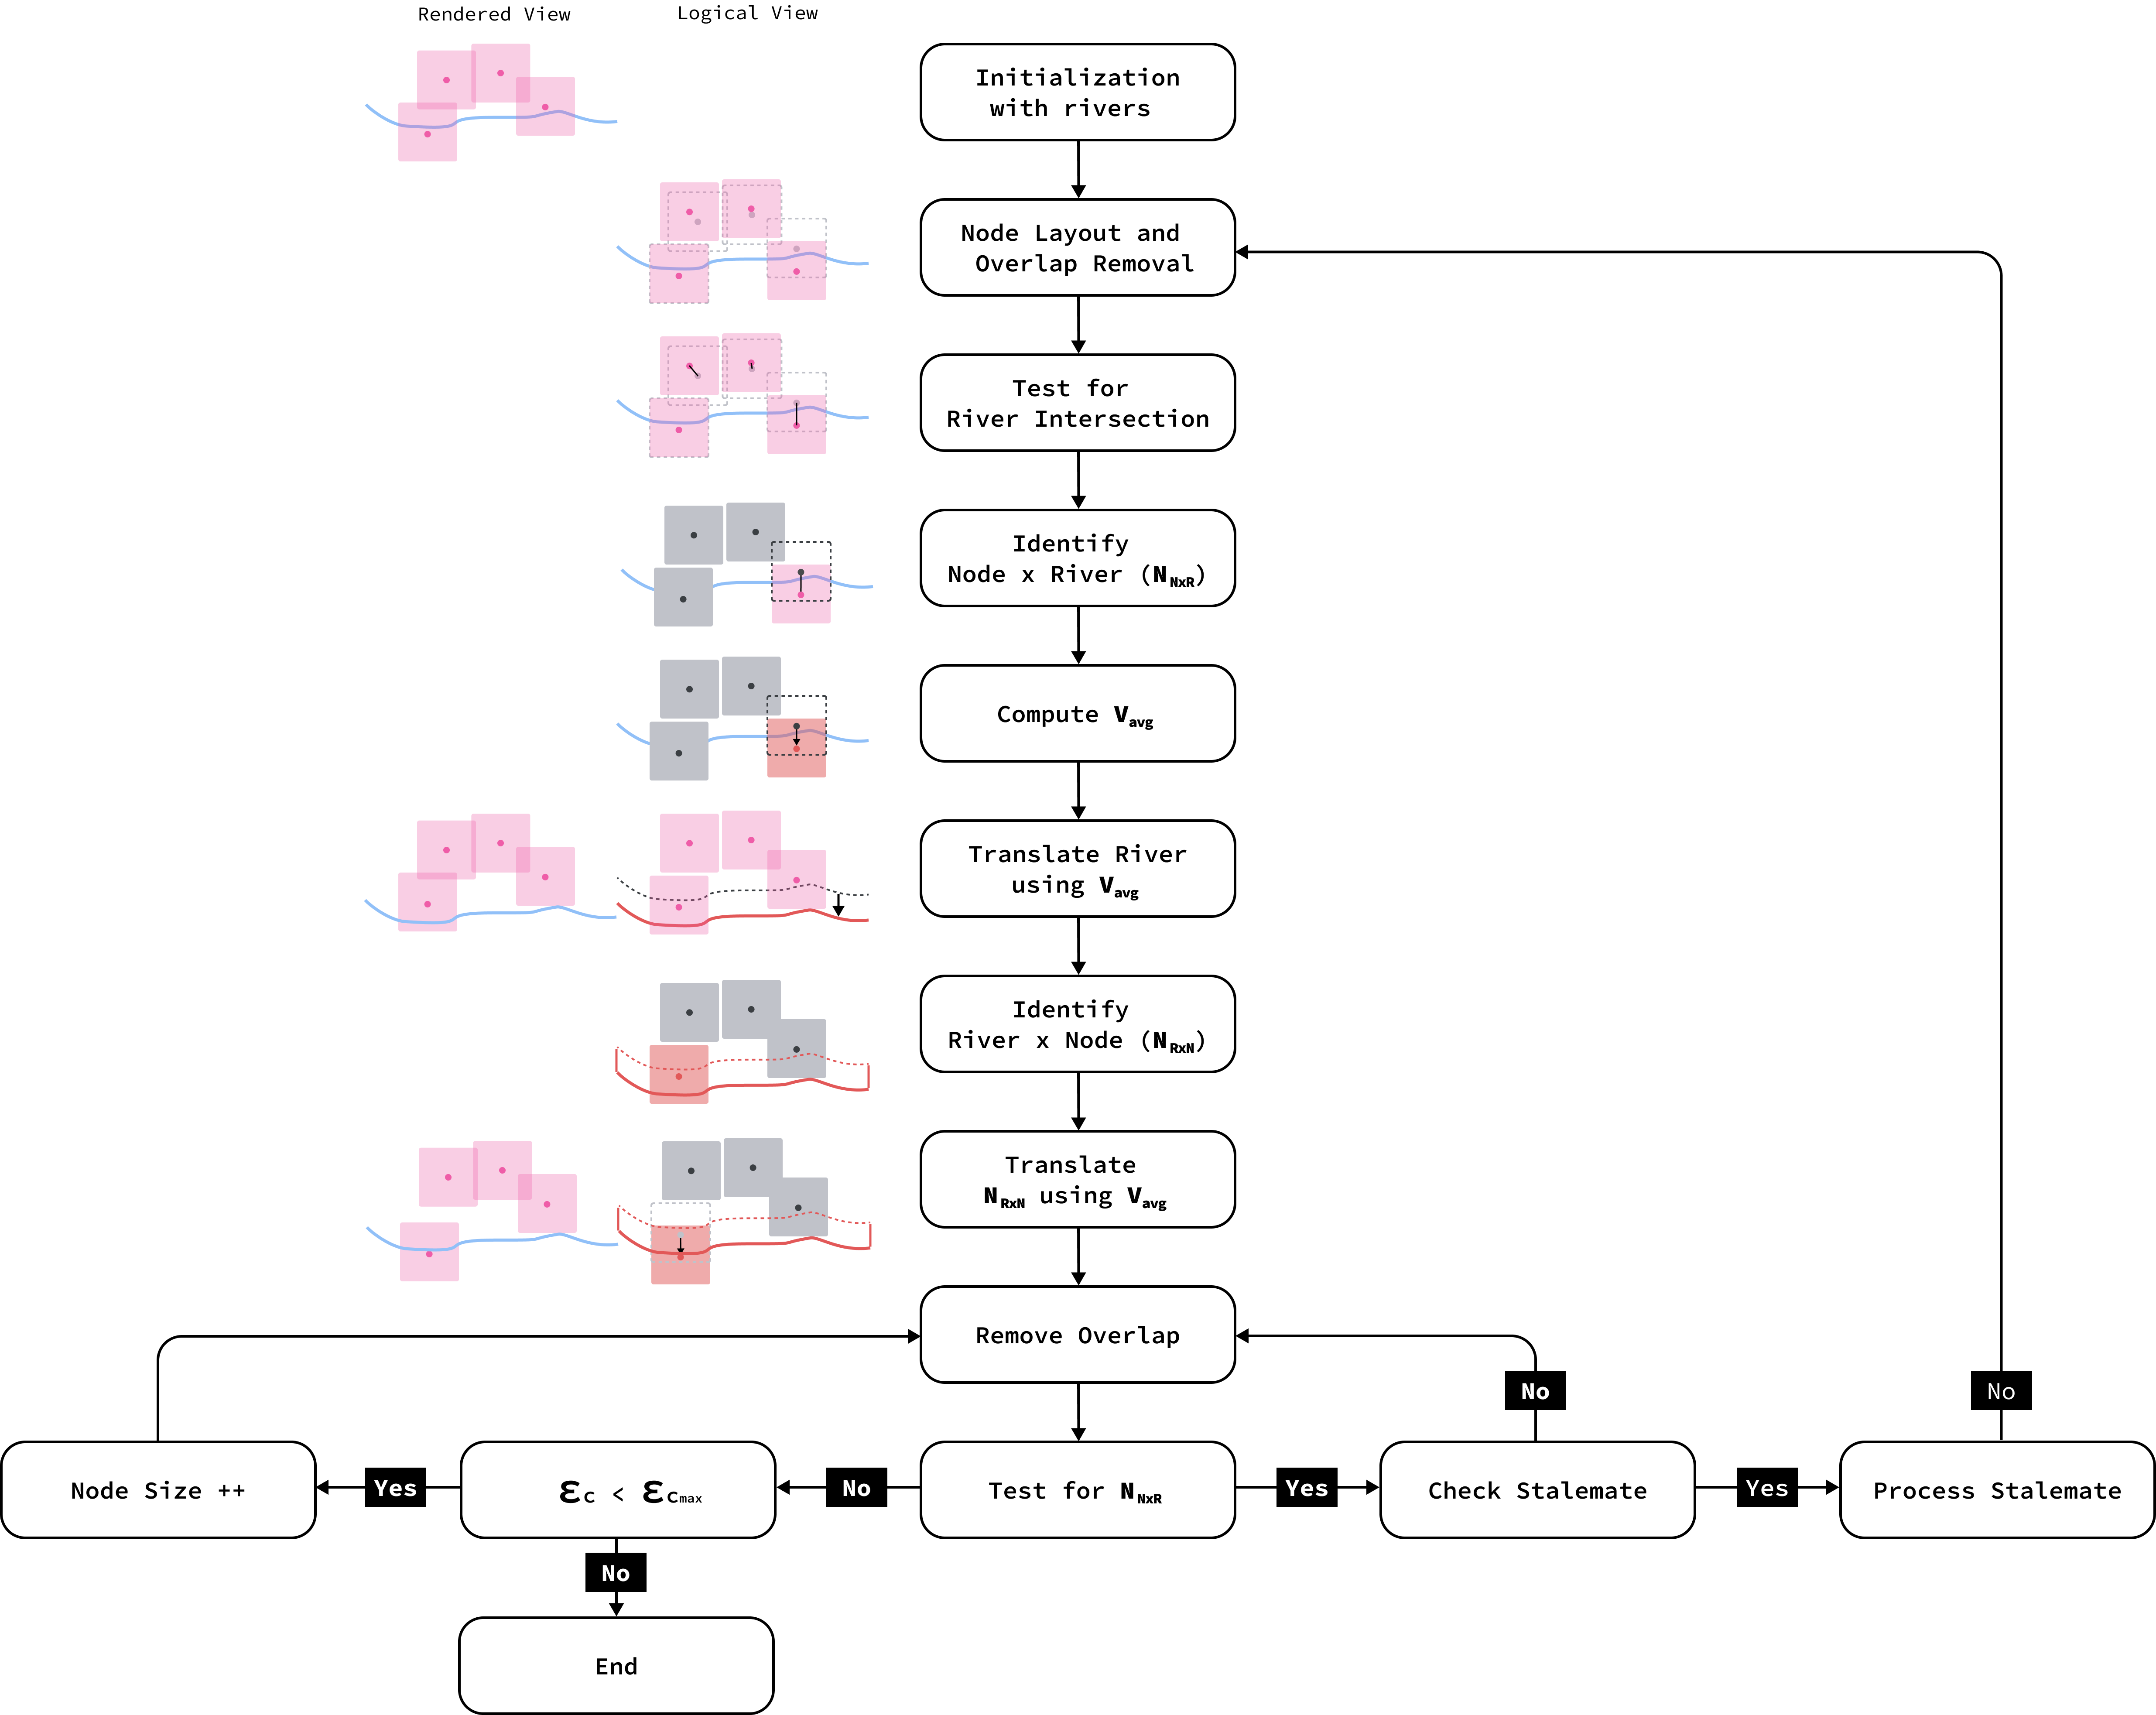
\includegraphics[width=0.8\textwidth,height=\textheight,keepaspectratio]{flowchart.png}
        \caption{An overview of our hybrid layout algorithm incorporating rivers.
            See also \Cref{alg:UpdateLayout} in Section \ref{sec:main} for more detail.
            See \Cref{fig:flowchart-stalemate} for the logic of processing a stalemate.
            For illustration purposes, we show the rendered views alongside the logical views representing the actual computation.}
        \label{fig:flowchart}
    \end{figure*}
}

{
    \begin{figure}[tb!]
        \centering
        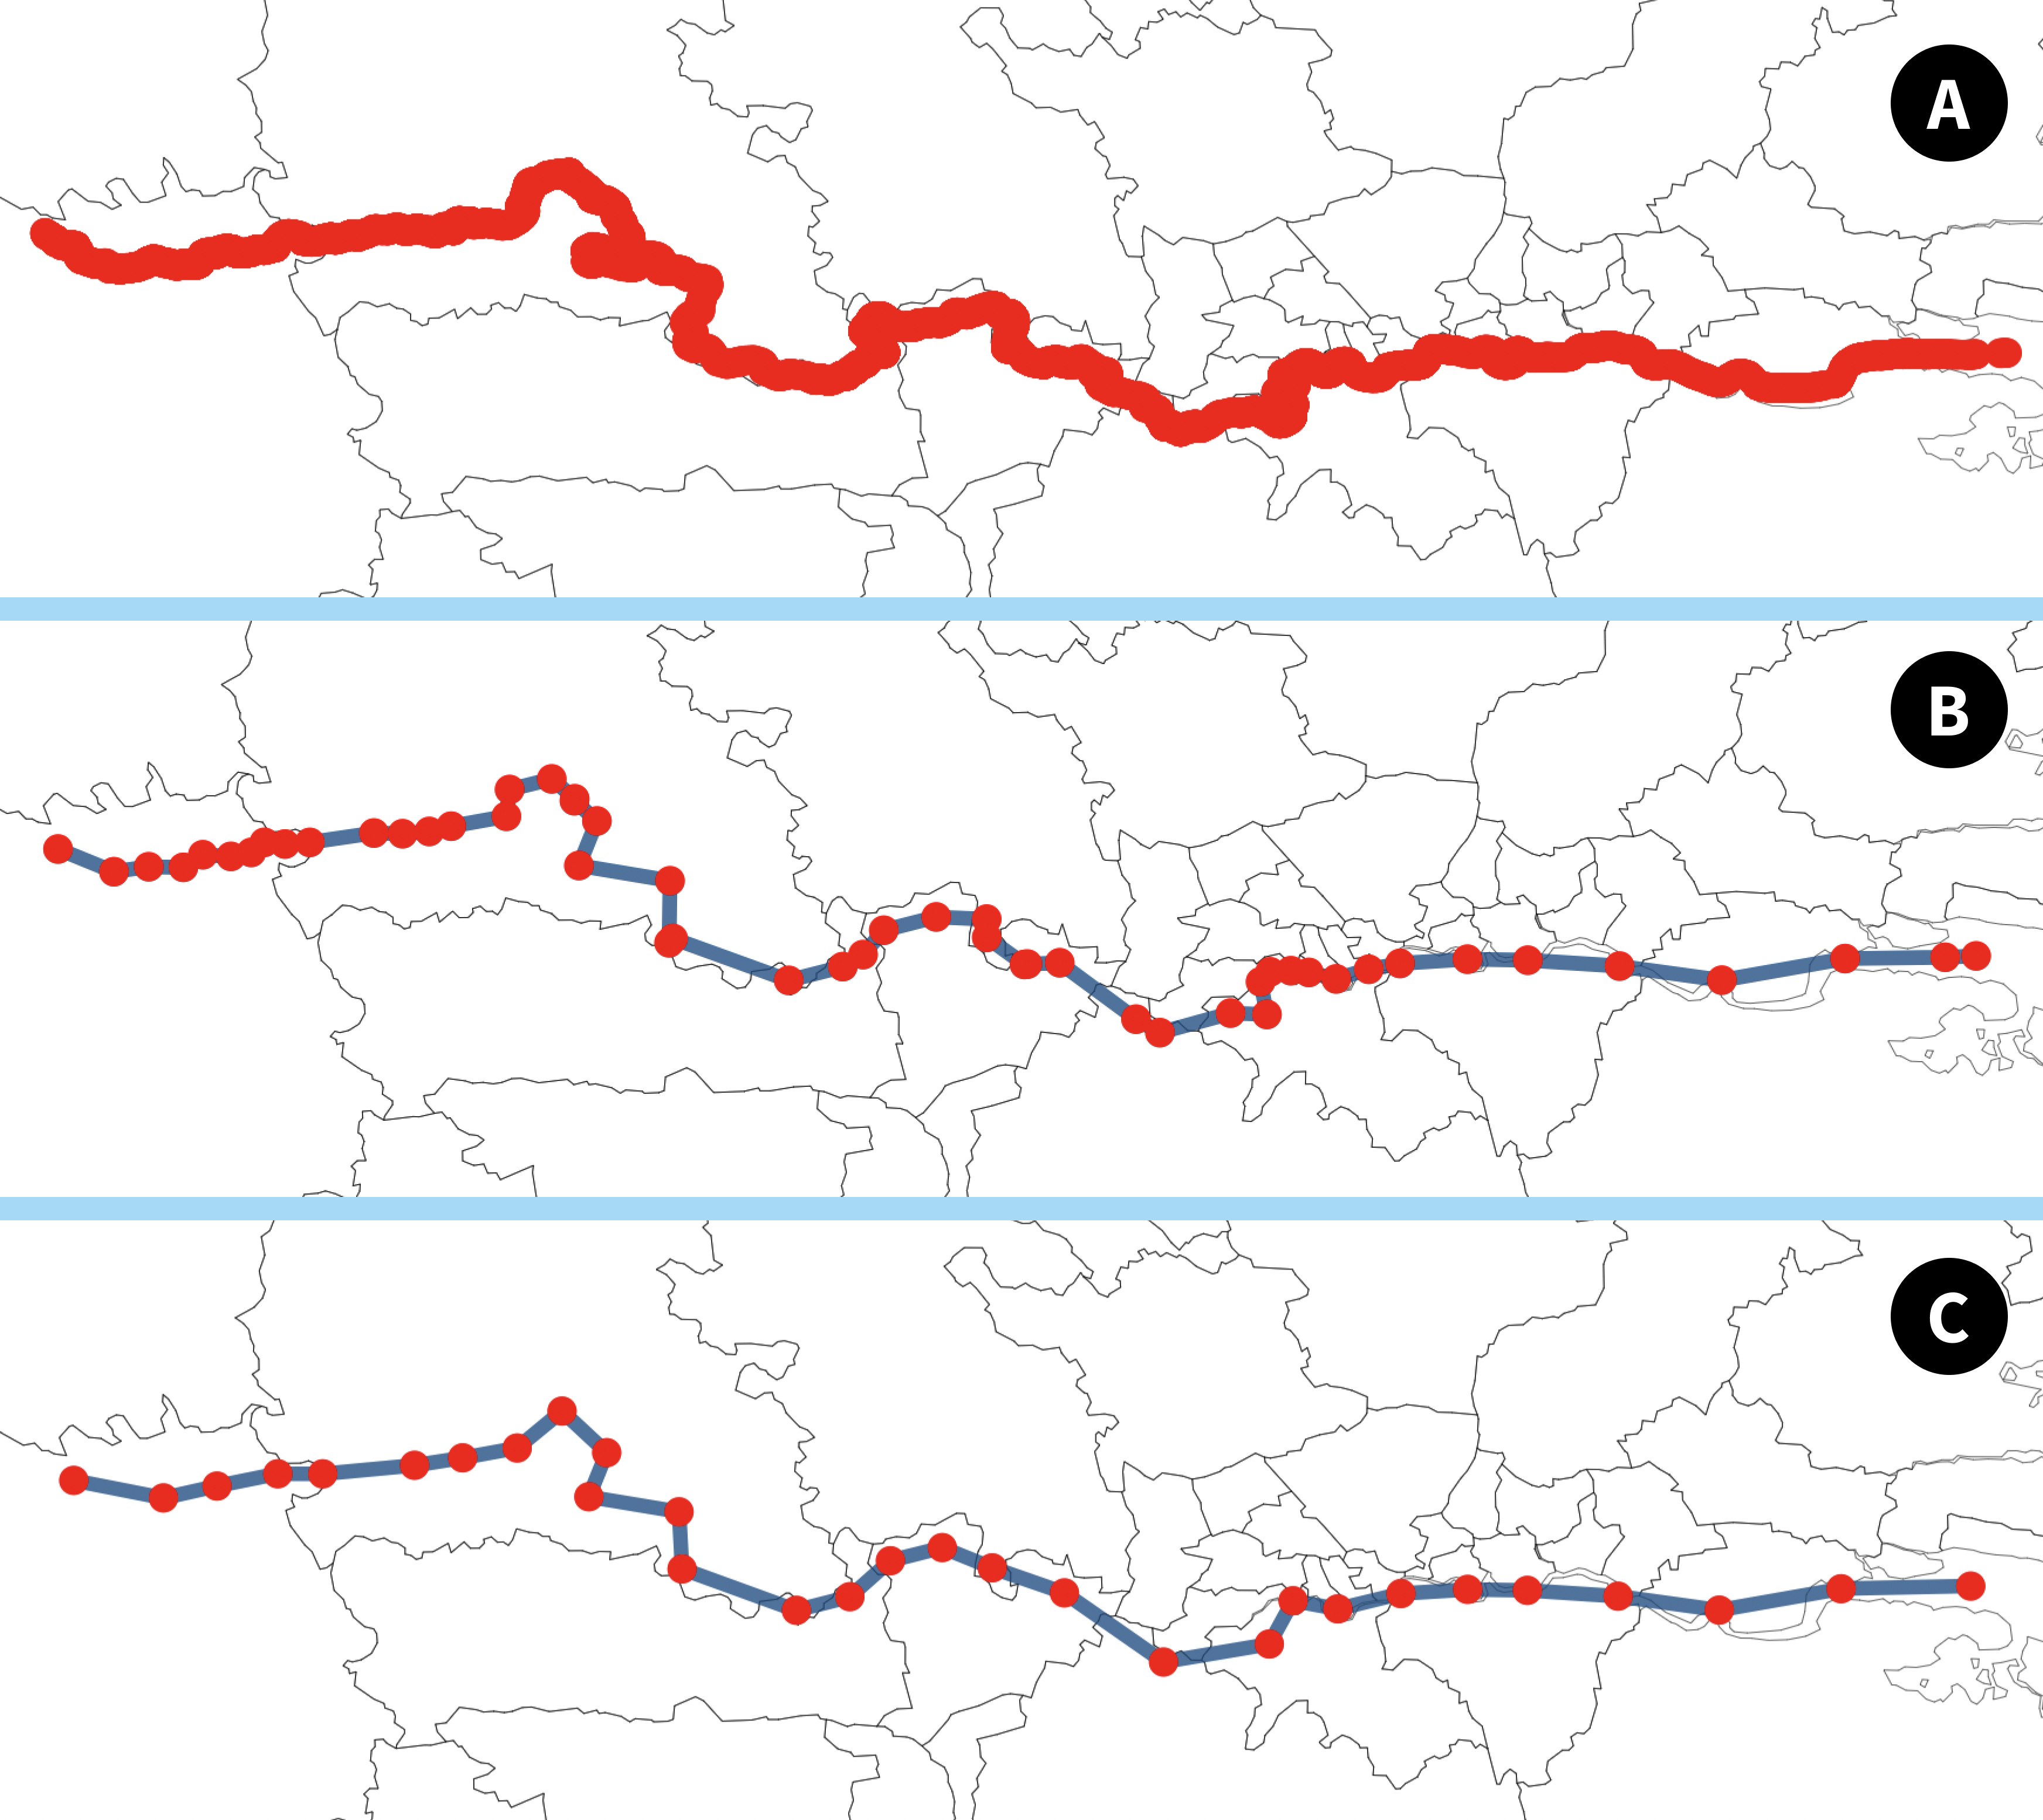
\includegraphics[width=0.8\columnwidth,keepaspectratio]{river_resolution.png}
        \caption{The resolution of rivers can be dynamically adjusted by the user.
            (A) shows River Thames at its original resolution with 10,170 edges.
            (B) shows the river at a reduced resolution of 49 edges.
            We further smooth the river by removing 19 vertices in dense areas, as shown in (C).
            The reduced resolution preserves the majority of River Thames' original shape and improves the performance of our river intersection tests.}
        \label{fig:river resolution}
    \end{figure}
}

\Cref{alg:UpdateLayout} and \Cref{fig:flowchart} provide an overview of the hybrid cartogram layout process that includes rivers.

\subsection{Initialization with Rivers}

We first load and (optionally) render the CCG geospatial boundaries.
For each CCG we compute the centroid and represent it using a square node, $ \node $, with the initial size, $ \nodeSize $ =1 pixel.
We then load the river shapefiles and render the rivers.
Since the vertices of the river in the shapefiles are not in sequential order, we first render the starting vertex, followed by the next nearest vertex.
We do not need the original river resolution to incorporate them into cartograms.
We reduce their resolution to match that of the cartogram nodes in order to facilitate node-river intersection tests.
This rendering approach enables us to adjust the river resolution as shown in \Cref{fig:river resolution}.
We further apply simplification by removing vertices that are too close to each other.
The initialization procedure is a one-time process that can be saved for reuse.


\subsection{Node Layout and Overlap Removal}

We first apply the Fast Node Overlap Removal (FNOR) algorithm that solves the Variable Placement with Separation Constraints (VPSC) problem \cite{dwyer2006Fast} in order to remove overlap between square nodes.
We chose FNOR over other node overlap removal algorithms because FNOR is capable of minimizing spread and node movement while maintaining a good level of global shape preservation \cite{chen2020Node}.
Initialized with a pixel size of unity, we gradually increase the node size by one unit at a time to ensure smooth transitions.
An increase in $ \nodeSize $ can cause the nodes to overlap.
During overlap removal, we compute node trajectories (See \Cref{alg:TranslateNode}) and translate nodes to their new position.
Nodes that cross a river, denoted $ \NxR $, are translated back to their previous position.
If a node oscillates across a river, we identify this as a stalemate.
One iteration of the layout ends when 1) no node overlap is present; AND 2) no nodes cross a river.
We then increase $ \nodeSize $ by one unit and repeat the algorithm until the average cartographic error, $ \nodeCartographicError $, a measure set by the user, reaches its maximum value $ \nodeCartographicErrorMax $.
The gradual size increase process provides stability to the layout, as can be seen in the accompanying video.

\subsection{River Intersection Testing}
\label{subsec:{River Intersection Testing}}

The logic for translating the position of a node is detailed in \Cref{alg:TranslateNode}.
When a node's position changes, we test if the node's trajectory intersects any segment of a river.
See \Cref{alg:check river intersection}.
A bounding box intersection test between the edge defined by node translation and river edges can be performed to reduce the number of edge intersection tests required.
Using the intersection test, we identify all nodes that cross the river as a result of the initial FNOR algorithm.
We label these nodes, $ \NxR $.

\subsection{Translating Rivers}
\label{subsec:{Translating Rivers}}

For all nodes $ \NxR $ that cross a river, $ \river $, we compute an average vector $ \vectorAvg $ used to translate $ \river $.
Whenever a node, $ \node $, crosses a river, we store a vector $ \nodeVectorNNn $ that points in the direction of the translation.
We then use a heuristic to translate $ \river $ using the average vector of node intersection $$ \vectorAvg = \sum_{i=1}^{\nodeTopologicalError} \frac{\Vector{\node_i\node_{i_t}}}{\nodeTopologicalError} $$, where $ \nodeTopologicalError $ is the number of nodes intersecting the river.
This step intends to create space for the next iteration of node translation without crossing a river.
The detailed procedure for translating rivers is provided by \Cref{alg:TranslateRiver}.


When a river, $ \river $, is translated by $ \vectorAvg $, this can trigger a scenario where nodes are crossed by a translated river, denoted $ \RxN $.
As a heuristic, we also translate these nodes by $ \vectorAvg $.
The reasoning behind this is that $ \vectorAvg $ indicates which direction the river needs to be translated to create space for the nodes that are too crowded together.
In practice, $ \vectorAvg $ is multiplied by a scaling factor $ \propto\vectorAvg $.
Thus, we can influence how far $ \river $ is translated in each iteration of the layout algorithm.
We can use this to ensure smooth transitions between iterations.

\subsection{Process Stalemates}
\label{subsec:{Process Stalemates}}

As the FNOR always attempts to produce an optimal node layout where node distribution and translation are minimized, a node's translation path can repeatedly intersect a river due to congestion, creating a stalemate situation, as shown in \Cref{fig:stalemate}.
If a node is translated between two positions, $ \node $ and $ \nodeFNOR $, for $ \stalemateMax $ iterations (a user-adjustable parameter), we introduce a heuristic solution: constructing a corridor to alleviate congestion.
A corridor, $ \Corridor $, is a rectangle with a width of $ \CorridorWidth $ and a length of $ \CorridorLength $, formed by deriving two edges $ \EdgeParallelA $ and $ \EdgeParallelB $ such that $ \EdgeParallelA \parallel \EdgeParallelB \parallel \nodeLineNtNc $ (See \Cref{fig:corridor}C and D).
All nodes enclosed by $ \Corridor $ are then translated by $ \nodeVectorTC $ to alleviate the congestion (See \Cref{fig:corridor}E).
The procedure for constructing corridors is provided by \Cref{alg:derive corridor}.

{
\begin{figure}[tb!]
    \centering
    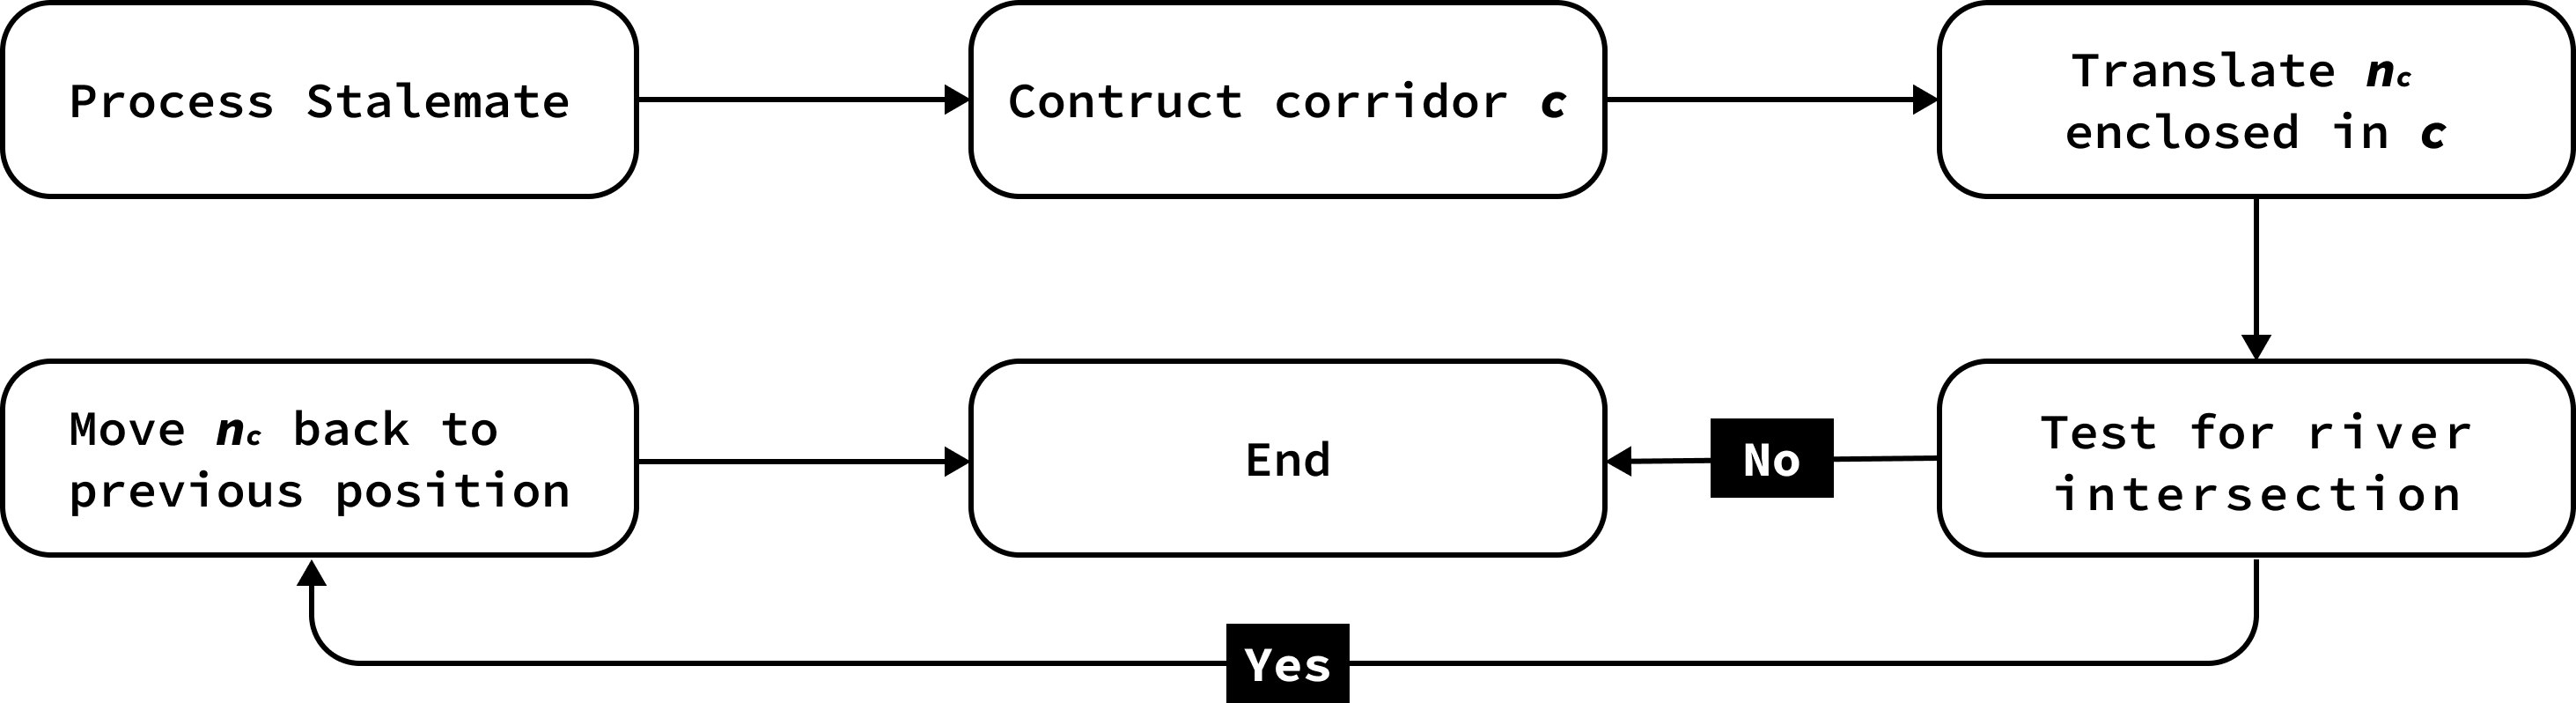
\includegraphics[width=\columnwidth,keepaspectratio]{flowchart stalemate.png}
    \caption{A flowchart illustration of stalemate processing.
    See \Cref{subsec:{Process Stalemates}}, \Cref{fig:stalemate}, and \Cref{fig:corridor} for more detail.}
    \label{fig:flowchart-stalemate}
\end{figure}
}

{
\begin{figure}[tb!]
    \centering
    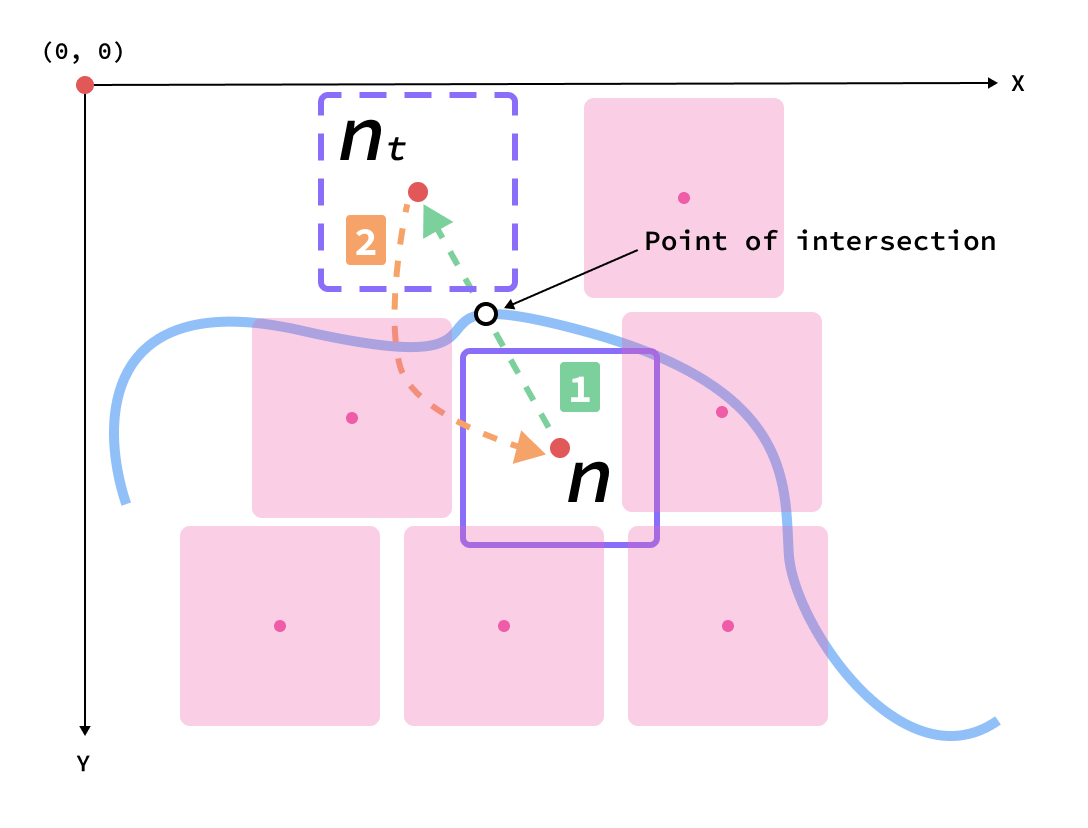
\includegraphics[width=\columnwidth,keepaspectratio]{stalemate.png}
    \caption{A stalemate: when a node's translation path $ \nodeVectorCT $ (iteration 1) intersects a river $ \stalemateMax $ times.
        The node is translated back to its previous position (iteration 2).
        A stalemate can occur when the area is congested and the node cannot translate to a new position without intersecting a river.}
    \label{fig:stalemate}
\end{figure}
}

{
\begin{figure}[tb!]
    \centering
    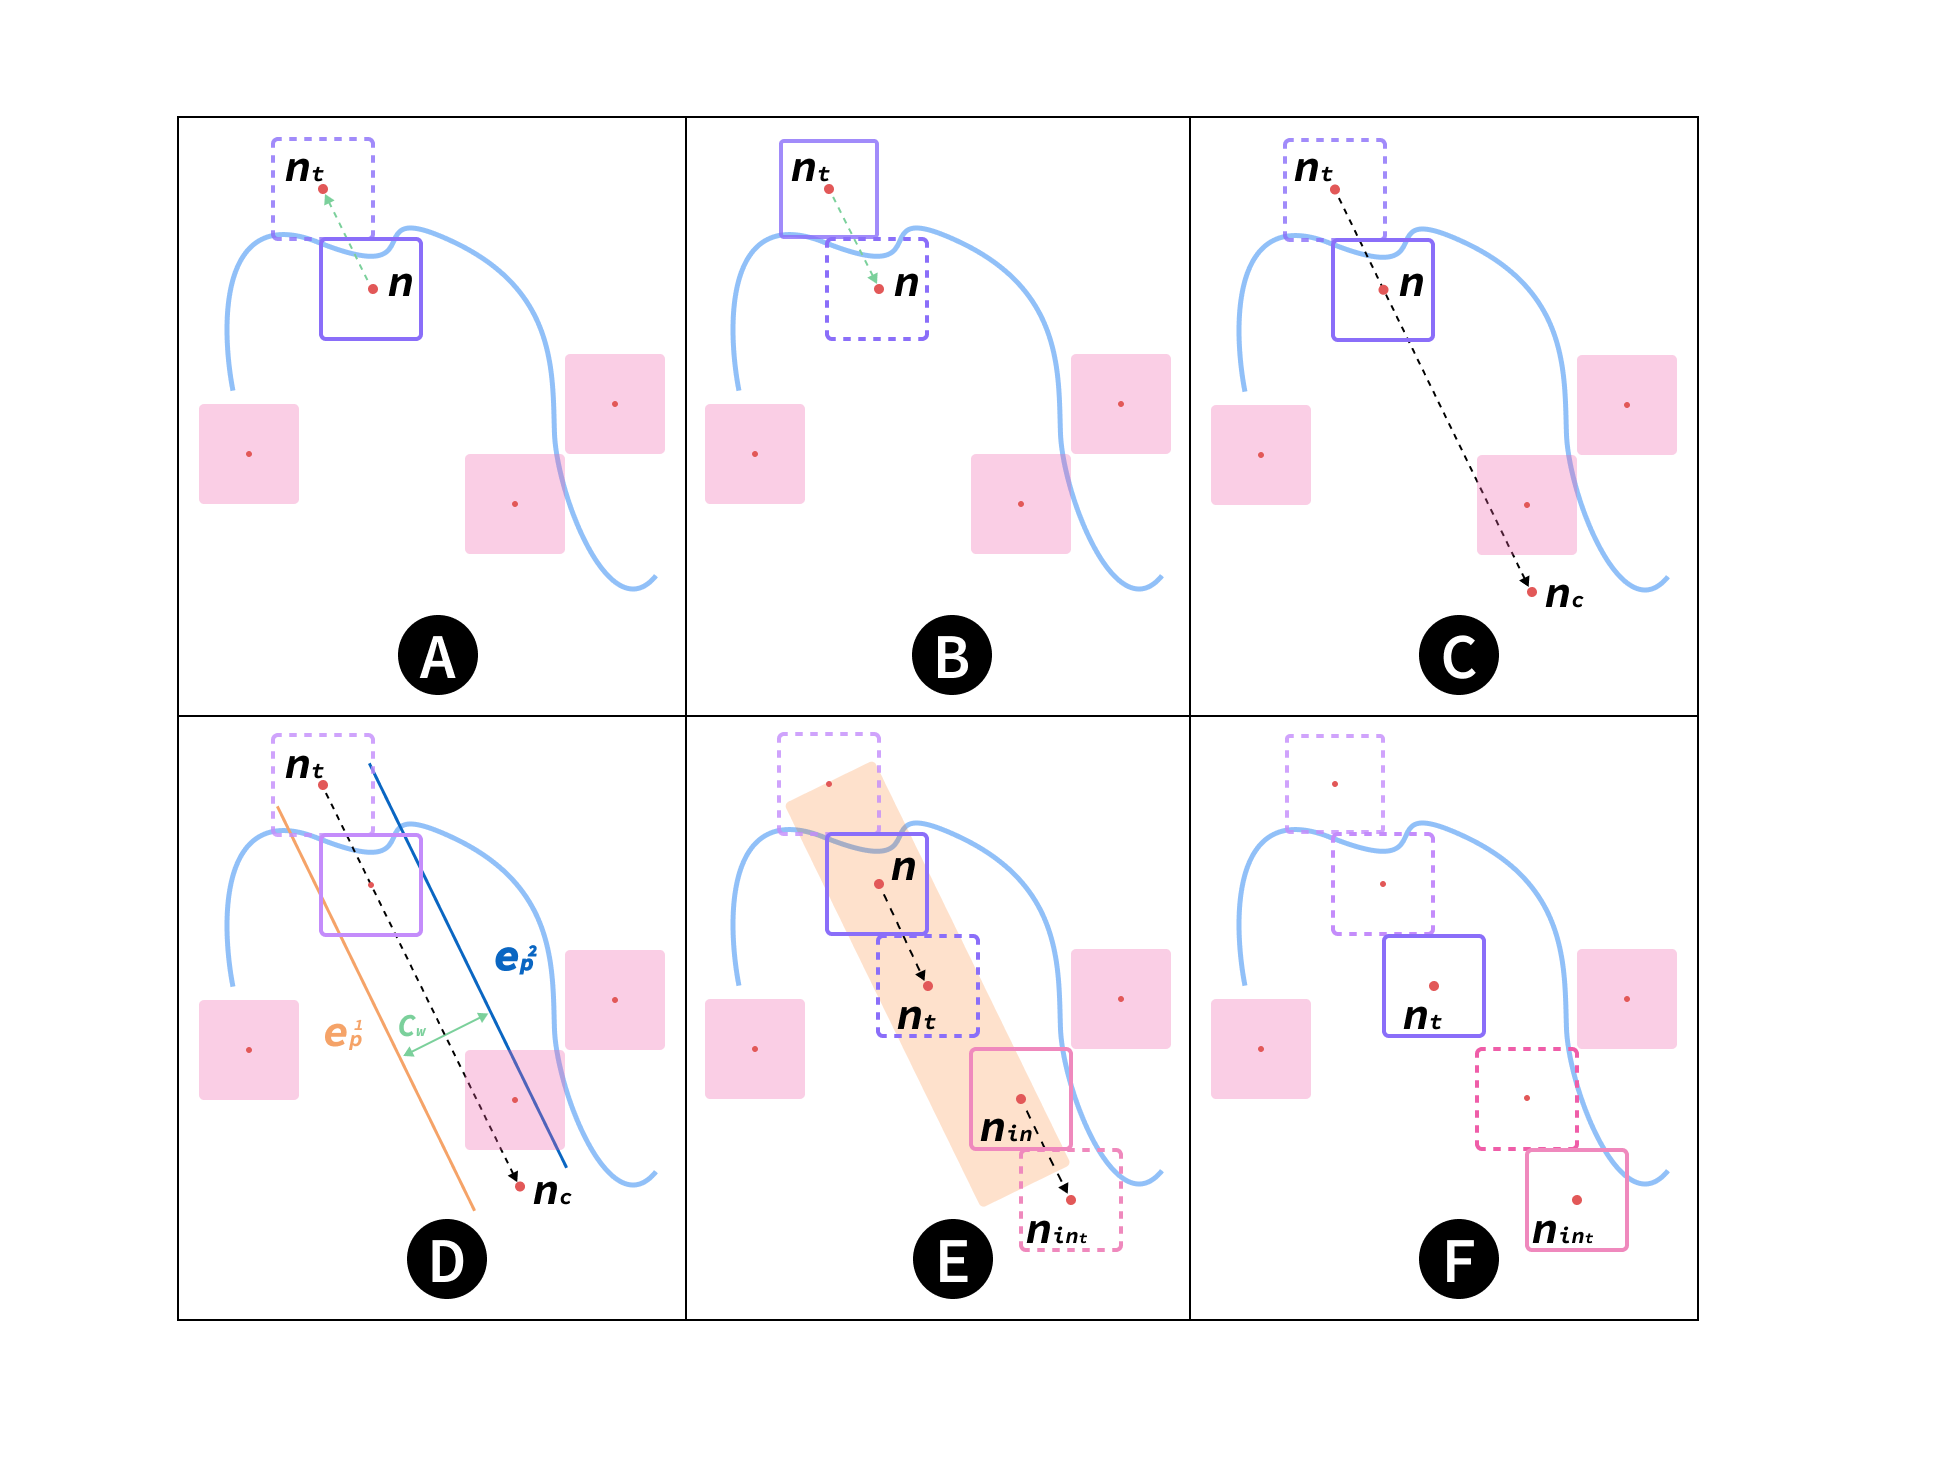
\includegraphics[width=\columnwidth,keepaspectratio]{corridor.png}
    \caption{A stalemate occurs when a node's translation path $ \nodeVectorCT $ intersects a river for $ \stalemateMax $ times, as shown in (A).
        To address this, we derive a corridor (orange rectangle in (E)) based on $ \node $ and $ \nodeFNOR $.
        All nodes within the corridor are translated based on $ \nodeVectorTC $, such that $ \nodeVectorNNn = \nodeVectorNinNinn $.
        For clarity in the illustration, we place nodes sparsely in this figure.}
    \label{fig:corridor}
\end{figure}
}


\subsection{Terminating the Algorithm}
\label{subsec:{Terminating the Algorithm}}

The algorithm terminates when $ \nodeCartographicError $ reaches $ \nodeCartographicErrorMax $, the error tolerance set by the user.
We adopt the maximum cartographic error from \citet{alam2015Quantitative}, namely: $$ \nodeCartographicErrorMax = \max _{\node \in \nodeList} \frac{|\node_i-\node_{i_t}|}{\max \{\node_i, \node_{i_t}\}}
$$

where $ \node_i $ and $ \node_{i_t} $ are the initial and translated regions in the cartogram, $ \nodeList $ represent the list of regions, and $ \nodeCartographicErrorMax $ is a normalized value that we express as a percentage.
For a detailed derivation of the formula, refer to the work by \citet{alam2015Quantitative}.
Because the algorithm processes node-river intersections, we can measure a novel kind of error, namely, topological error $ \nodeTopologicalError $.
We maintain $ \nodeTopologicalError = 0 $, however, we can count how many nodes would have crossed a river if we did not test for this and simply let nodes cross rivers.
We express $ \nodeTopologicalError $ in the normalized range $ \nodeTopologicalError \in [0,1] $, where $ \nodeTopologicalErrorMax $ is the case where all nodes cross a river.

When the algorithm terminates, the node layout is considered optimal where no nodes have crossed or crossed a river (denoted $ \nodeTopologicalError $ = 0 and $ \nodeCartographicError < \nodeCartographicErrorMax $).
Every node remains on the same side of the river as its centroid.

\subsection{User Options}\label{subsec:{UserOptions}}

\Cref{fig:overview} presents an overview of the application, including user options.
The user can adjust the following parameters:

\bobgraph{Rendering Visibility:} The rendering visibility of various elements, including the choropleth shapefile, rivers, nodes, and node centroids, can be toggled on and off.

\bobgraph{Node Mapping:} Both size and color of the nodes can be mapped to different EHR attributes or set to uniform.

\bobgraph{Overlap Removal Speed:} The overlap removal process can be observed in a step-by-step manner, or the algorithm can be run automatically.

\bobgraph{Maximum Cartographic Error:} The user can adjust the maximum cartographic error, $ \nodeCartographicErrorMax $, which is used to terminate the algorithm.

\bobgraph{River Translation:} The behavior of rivers during the process can also be adjusted by the user: 1) Enable river crossing: this option allows nodes to cross rivers.
Nodes cannot cross rivers by default; 2) Disable river translation: this option disables the translation of rivers, rivers are translated by default.
Both options are useful for generating different layouts and to observe the behavior of the hybrid layout algorithm.

\bobgraph{Corridor Length:} The user can define the length of a corridor that is used to resolve stalemate situations.
A longer corridor length allows more nodes to be translated when a stalemate occurs, but may result in a less accurate layout.
The default corridor length is three times the max node size.

\bobgraph{River Thickness and Resolution:} Increasing the thickness of rivers may improve the recognizability of the cartogram.
Similarly, increasing the resolution of rivers, at the expense of the speed of node-river intersection test, may produce a layout with higher legibility.

    {
        \begin{figure*}[tb!]
            \centering
            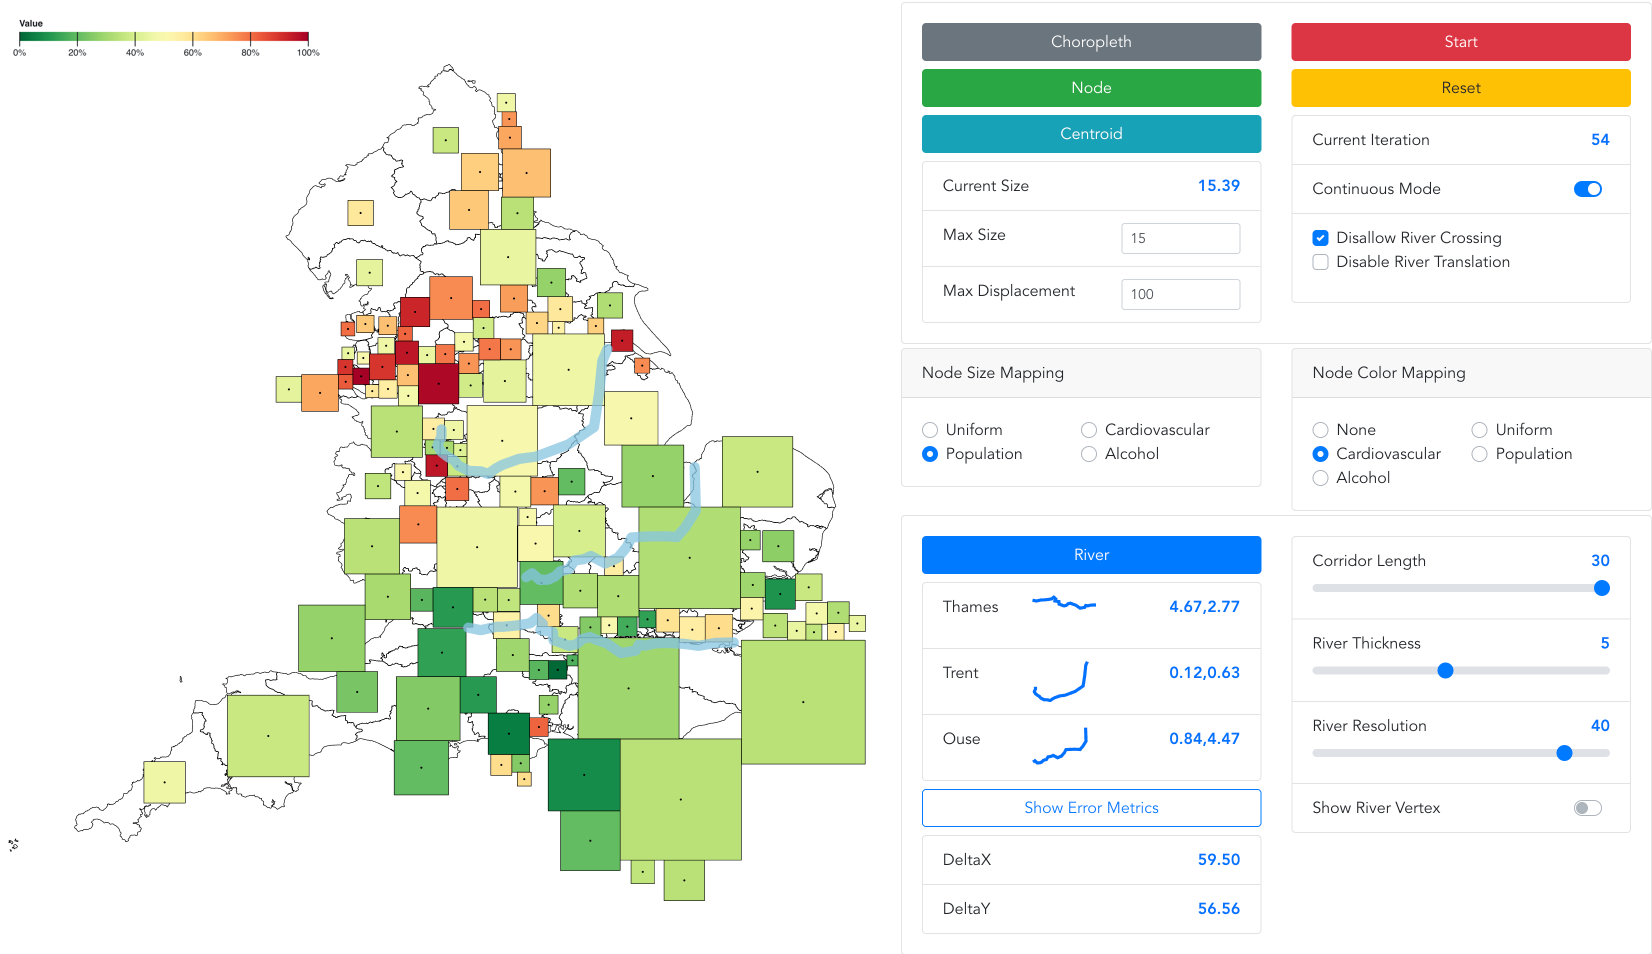
\includegraphics[width=0.9\textwidth,keepaspectratio]{UI.png}
            \caption{A screenshot of the user interface.
            User options are provided to adjust the terminating conditions (size and error), color mapping, visibility of nodes and rivers.
            Other options include the ability to control the overlap removal behavior: rivers can be static or dynamic.
            See \Cref{subsec:{UserOptions}} for more on user options.
            In this figure, $ \nodeCartographicErrorMax $ = 1.875\%, and an $ \nodeTopologicalError $ of 9.63\% is eliminated.}
            \label{fig:overview}
        \end{figure*}
    }

\newcommand{\pCount}{24 }
\section{User-Centered Evaluation}\label{sec:{User-Centered Evaluation}}

We conduct a within-subject user study to evaluate the effectiveness of our approach.
We chose this type of evaluation because legibility is a human-centred characteristic.
Many different types of statistical error metrics have been evaluated in previous work \cite{nusrat2016State}, however, our focus is more user-centric in nature.

\subsection{Study Hypothesis}\label{subsec:{Study Hypothesis}}

We formulate the following hypotheses to motivate our user study:

\textbf{H1:} The introduction of rivers can improve the legibility and recognizability of cartograms.

\textbf{H1.1:} The introduction of rivers can increase the accuracy of the target location.

\textbf{H1.2:} The introduction of rivers can reduce the time required to locate a target region in a cartogram.

We test these hypotheses using location-based tasks.
Given a standard choropleth on the left side of the screen and the corresponding cartogram on the right side, we ask user study participants to locate the given region in the choropleth (on the left) in the cartogram (on the right).
See \Cref{fig:task}.

\subsection{User Study Variables}\label{subsec:{User Study Variables}}

In this section, we discuss the variables of our user study.

\bobgraph{Independent Variables: }The primary independent variable is the presence of rivers in the cartograms, which directly impacts the final layout of the cartogram. 
The identical set of rivers is either rendered or hidden collectively.

\bobgraph{Dependent Variables: }\textit{Accuracy:} Given a CCG location in the choropleth on the left, we ask the participant to locate the corresponding node in the cartogram.
Accuracy as the primary dependent variable is measured by the number of correct CCGs located and chosen by the participants.
\textit{Response time:} Another dependent variable is the time it takes the participants to complete each task.

\bobgraph{Control Variables: }\textit{Choice of color map:} We use D3's built-in interpolateRdYlGn color map, a color scheme of red, yellow, and green, to depict the data in our cartograms.
\textit{Communicating the target CCG to the user:} We inform the participant about the target CCG they need to find.
The target CCG is shown in the form of a nonstop blinking (between its original color and black) area on the screen, each blink is given a duration of 2 seconds.

\subsection{User Study Design}\label{subsec:{User Study Design}}

In this section we describe the user study participants, datasets, and the experimental procedure.
The study was approved by the University of Nottingham's Research Ethics Committee (Ref: 2021-2022-001).

\bobgraph{Participants:} We recruited \pCount participants.

\begin{itemize}
    \setlength\itemsep{0px}
    \item Gender: 10 females and 14 males
    \item Age Group: 18-24 (16), 25-29 (8)
    \item Education: 1 PhD, 11 Master's, 8 Bachelor's, 4 Others
\end{itemize}

\bobgraph{Datasets:} We used the following EHR datasets for our evaluation:

\begin{itemize}
    \setlength\itemsep{0px}
    \item Population
    \item Under 75 mortality from cardiovascular disease
    \item Emergency admissions for alcohol-related liver disease
    \item Alcohol-specific admission and readmission
\end{itemize}

135 CCGs are rendered on the screen as a choropleth on the left.
We then generated another view on the right using cartograms.
The color of both visual designs is mapped to a data dimension.
No cartograms were used more than once per participant.
See \Cref{fig:task} for an example.

    {
        \begin{figure}[tb!]
            \centering
            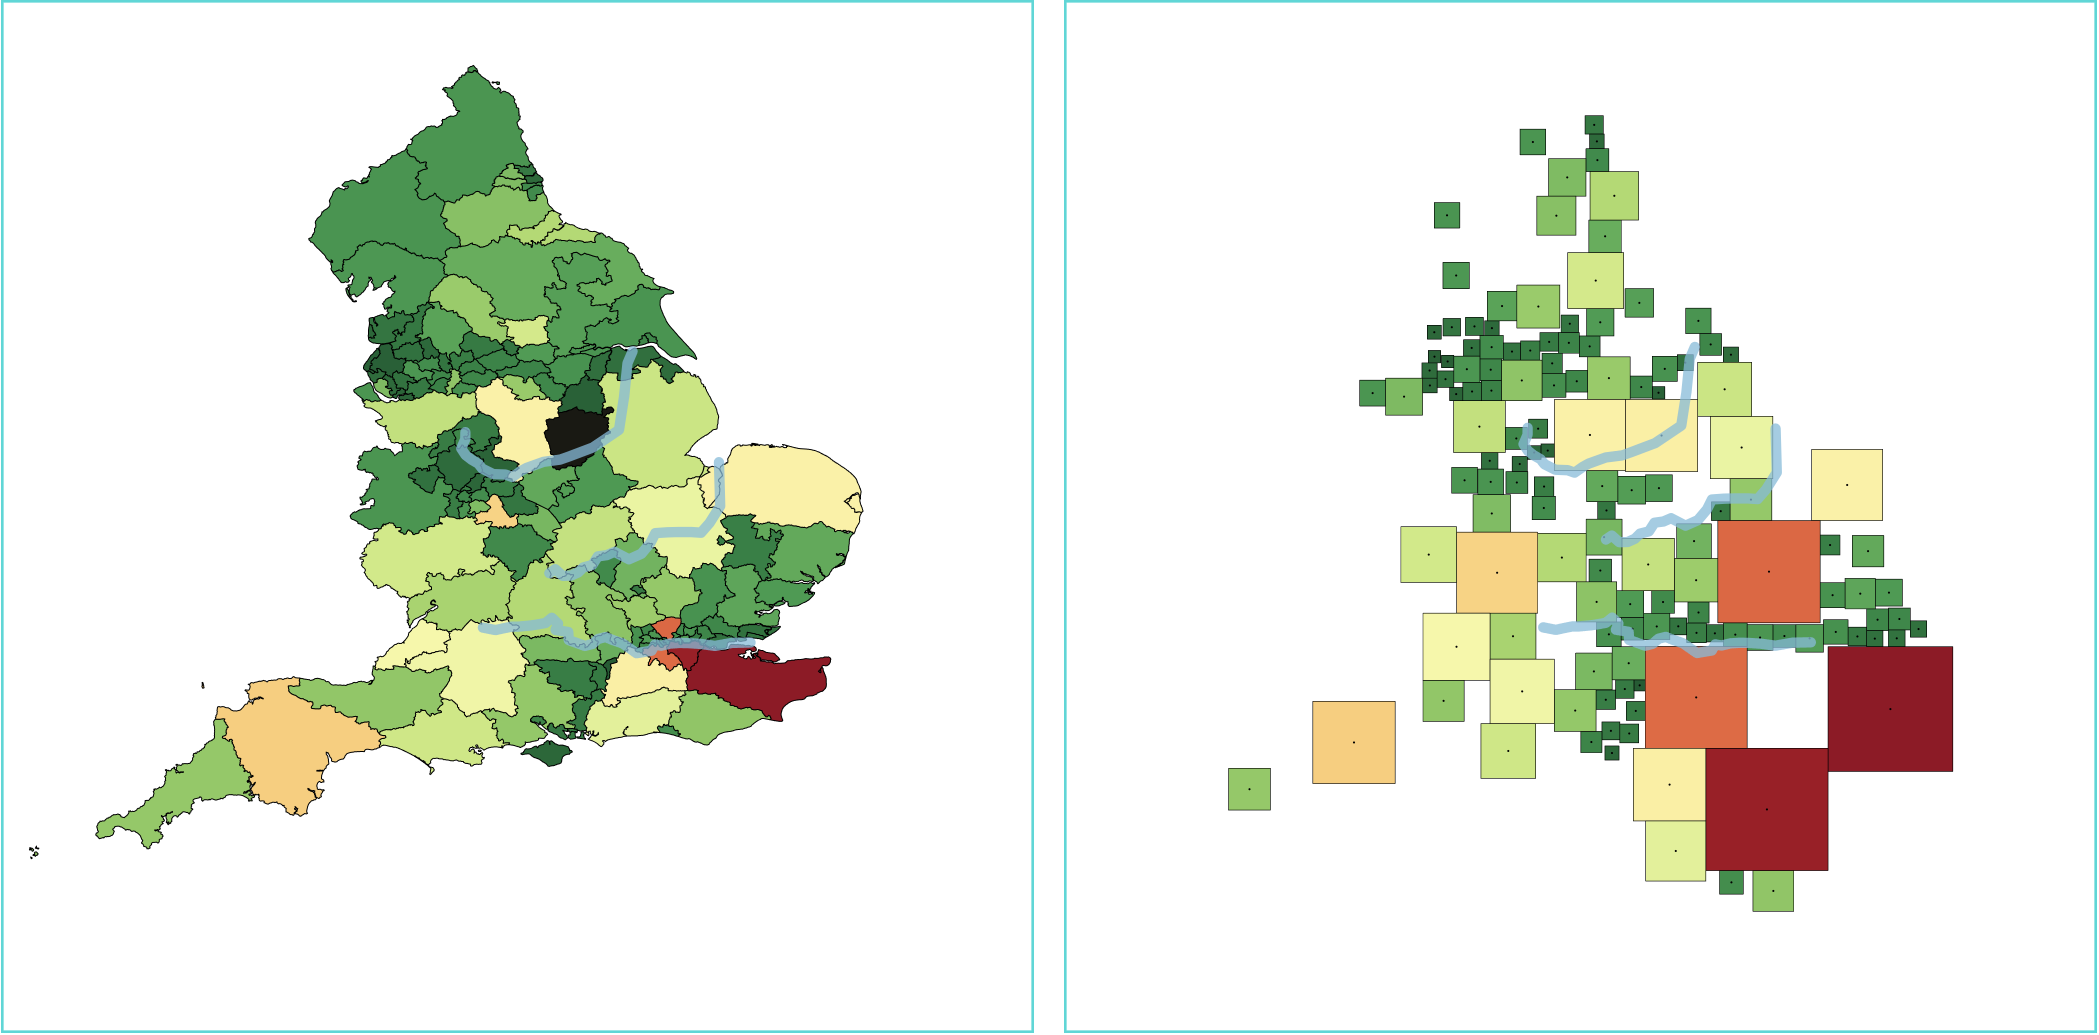
\includegraphics[width=\columnwidth,keepaspectratio]{task.png}
            \caption{A sample location task for participants.
                The left shows the choropleth map, and the right shows the corresponding cartogram.
                Both images show the three longest rivers in England, and color is mapped to CCG population.
                The target CCG blinks on the choropleth (shown in black), and participants are asked to identify this CCG on the cartogram.
                In this figure, $ \nodeCartographicErrorMax $ = 1.875\% , and an $ \nodeTopologicalError $ of 6.67\% is eliminated.
            }
            \label{fig:task}
        \end{figure}
    }

\subsection{Procedure}\label{subsec:{Procedure}}

Due to pandemic restrictions, we designed the user study to be carried out online.
Participants are expected to use their retail hardware for the tasks.
However, devices with small screens are not recommended because of the large size of the cartograms that are rendered.
The within-subject user study includes four parts:

\textbf{P1:} The participants are asked to listen to instructions and training provided as both text and videos.
The instructions are designed to help participants understand the concepts used in the tasks.
An instructional video was provided \footnote[1]{Instructional video: \url{https://www.youtube.com/playlist?list=PLL7sHvxLtD75fMtrUQrAdddjt3wfFkcWz}}.

\textbf{P2:} The participants are given three practice tasks to familiarize themselves with the user study design.
A sample task \footnote[2]{A sample task is accessible at \url{https://ghr.wangqiru.com/#/P1}.} is shown in \Cref{fig:task} and included in the online materials\footnotemark[3].
The practice tasks are identital to the actual tasks, accompanied by instructions provided before the actual tasks commence.
The results from these practice tasks are not included in the final analysis.
These tasks also serve as a quality test to see whether users are taking the study seriously.
A demonstration of three sample tasks is also included in the instructional video\footnotemark[1].

\textbf{P3:} The participants are asked to complete 16 location tasks that involve 4 target CCGs.
See the online materials for exact locations of target CCGs\footnotemark[3].
Response and reaction time are recorded.
These 4 CCGs are selected to avoid extreme cases (thus bias the result), in terms of size, color, and location.

\textbf{P4:} The participants are asked to complete a questionnaire\footnote[3]{The materials for P1-P4 are available on the Open Science Foundation website at \url{https://osf.io/q39w7}.} that consists of 5-Point Likert Scale questions and open-ended questions.



\subsection{User Study Results}
\label{subsec:{User Study Results}}

{
\begin{figure}[b!]
    \centering
    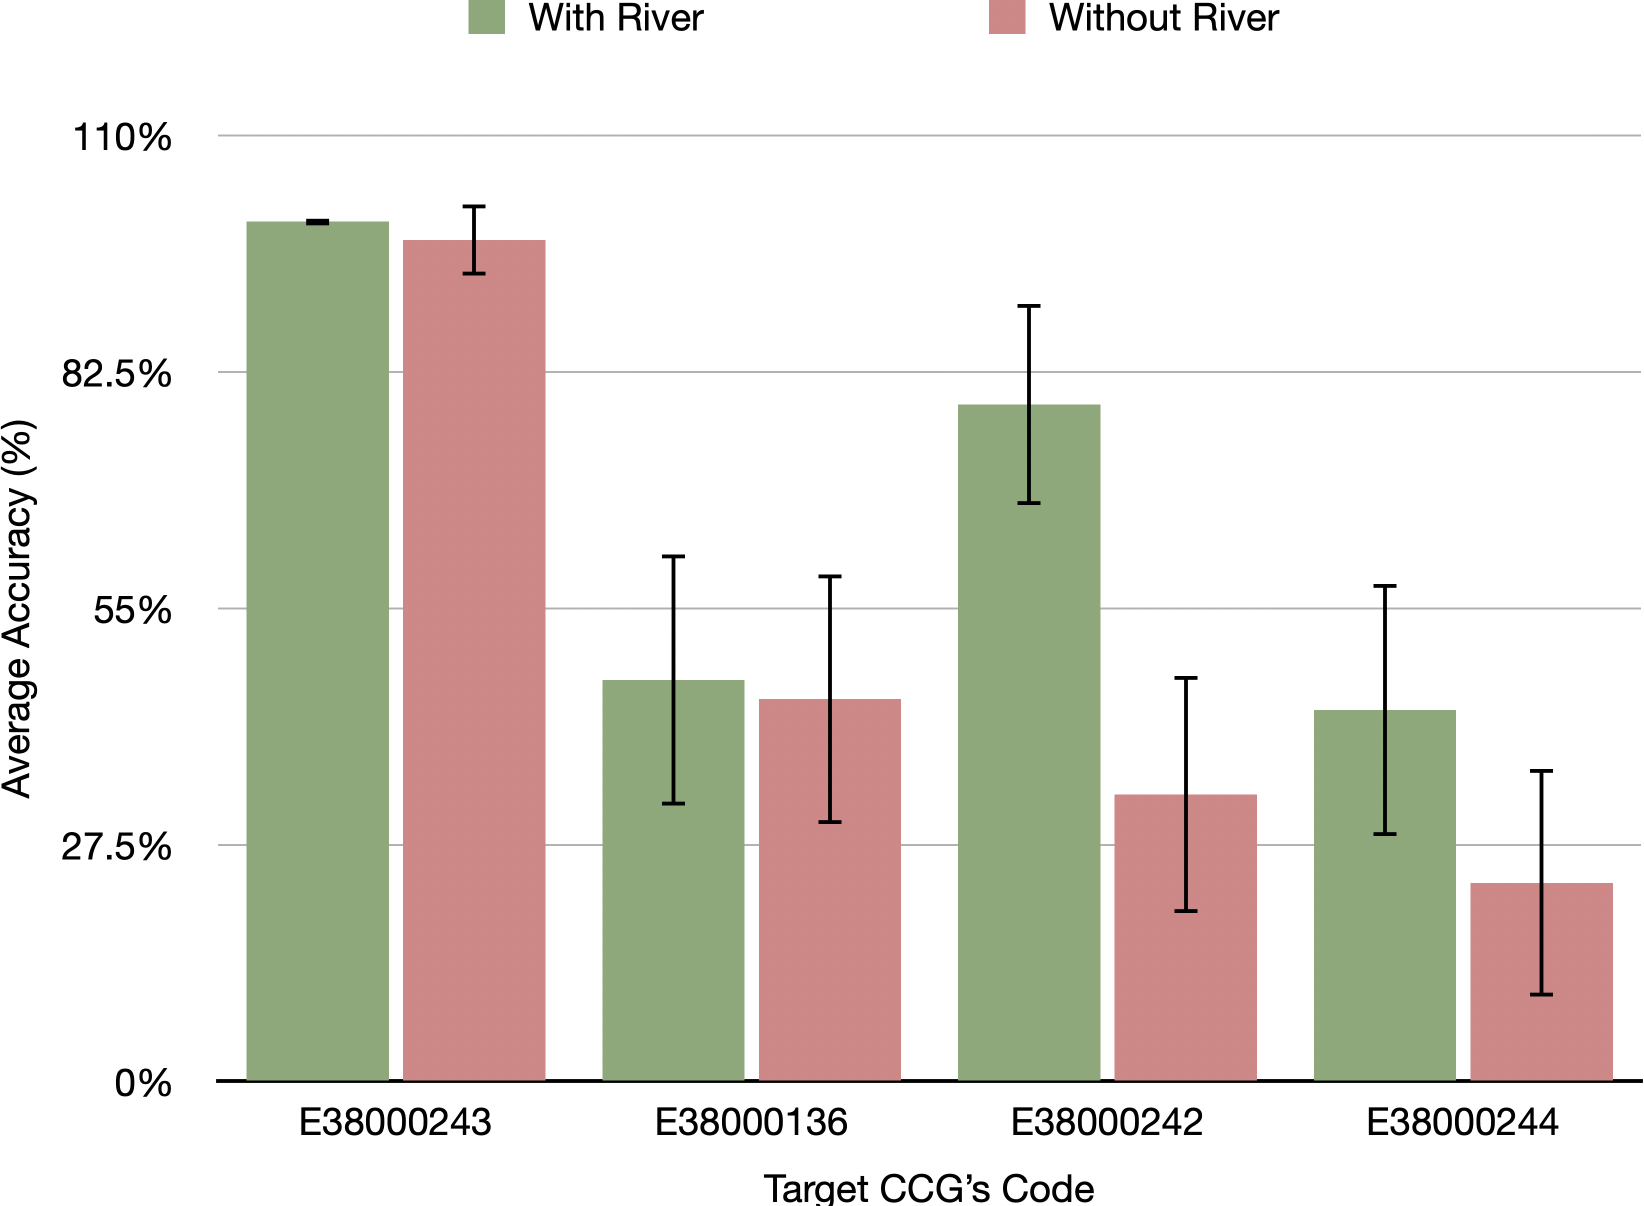
\includegraphics[width=\columnwidth,keepaspectratio]{accuracy.png}
    \caption{In the bar chart, the y-axis shows the average accuracy rate of locating CCGs with and without rivers for user study participants.
        The x-axis shows the four target CCGs, as described in Procedure P3.}
    \label{fig:task-acc}
\end{figure}
}


In this section, we delve into the analysis of the preliminary user study conducted.
Our study involved the recruitment of \pCount participants, each tasked with completing 16 location-related tasks.
As a result, we collected a total of 384 responses.
However, we excluded 24 responses from our analysis as they took over 60 seconds to complete.
We hypothesize that these prolonged response times indicate potential distractions experienced by participants during the study.

\bobgraph{Accuracy:} \Cref{fig:task-acc} shows the accuracy measured by the number of correct CCGs chosen by the participants.
The chart shows that the introduction of rivers has improved the accuracy of two CCGs.
The accuracy for the two groups differs significantly according to the two-sample unequal variance $t$-test performed, $t$(262.98) = 3.76, $p$ = 0.0002.
This supports our hypothesis H1.1 that the introduction of rivers increases target location accuracy.


\bobgraph{Response Time:} \Cref{fig:task-rt} shows the average time to locate a CCG measured for four CCGs.
The chart indicates that the introduction of rivers has slightly reduced the time needed to locate CCGs.
The two groups show no statistically significant differences according to the two-sample unequal variance $t$-test performed, $t$(356.03) = 0.87, $p$ = 0.38.
However, the average time to locate a given CCG is reduced for 3 out of the 4 CCGs users in the study.

    {
        \begin{figure}[t!]
            \centering
            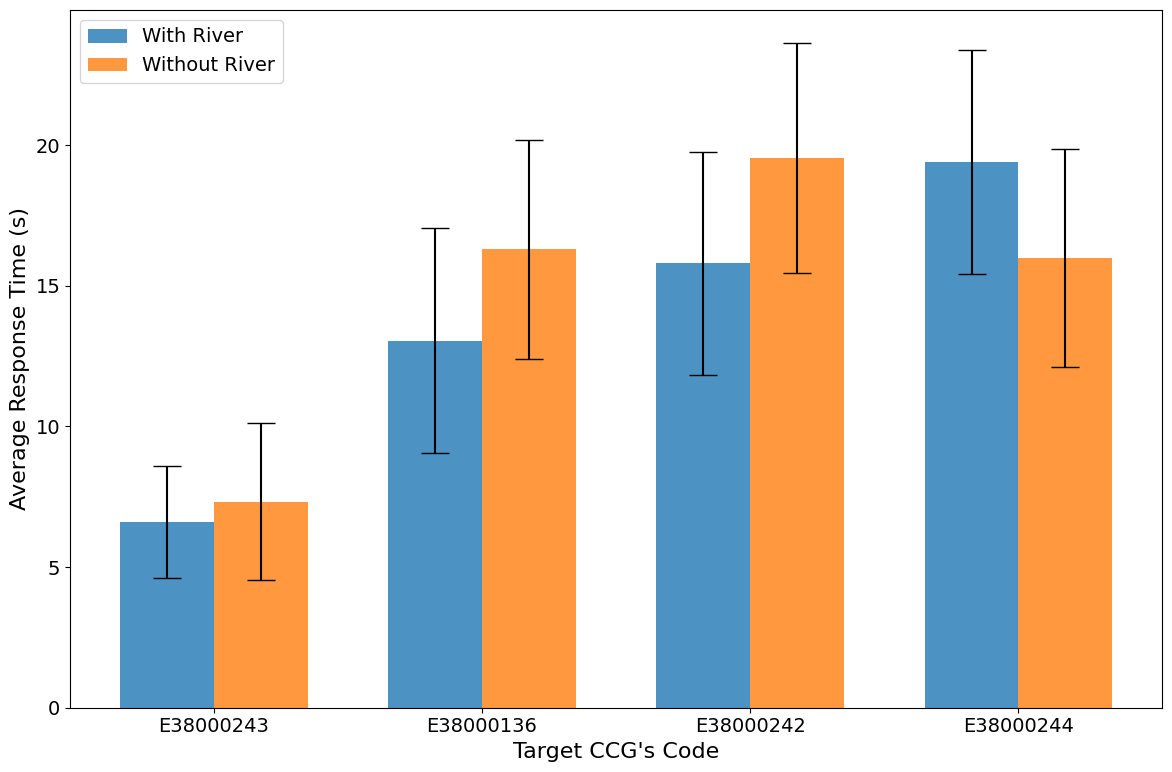
\includegraphics[width=\columnwidth,keepaspectratio]{rt.png}
            \caption{In the bar chart, the y-axis shows the average response time for locating CCGs with and without rivers for user study participants.
                The x-axis shows the four target CCGs, as described in Procedure P3.}
            \label{fig:task-rt}
        \end{figure}
    }

\bobgraph{Participant Feedback:} \Cref{fig:likert} shows the results of the following Likert Scale questions:
\begin{enumerate}[label=(\Alph*),align=left,leftmargin=*,labelindent=1em]
    \item 87.5\% of participants agree that including rivers is useful.
    \item 83.3\% of participants agree that rivers increase the legibility of a cartogram.
    \item 95.8\% of participants agree that including rivers makes cartograms easier to understand.
    \item 62.5\% of participants agree that including rivers makes CCGs easier to locate.
    \item 87.5\% of participants agree that including rivers adds value to the standard cartogram.
\end{enumerate}

{
\begin{figure}[tb!]
    \centering
    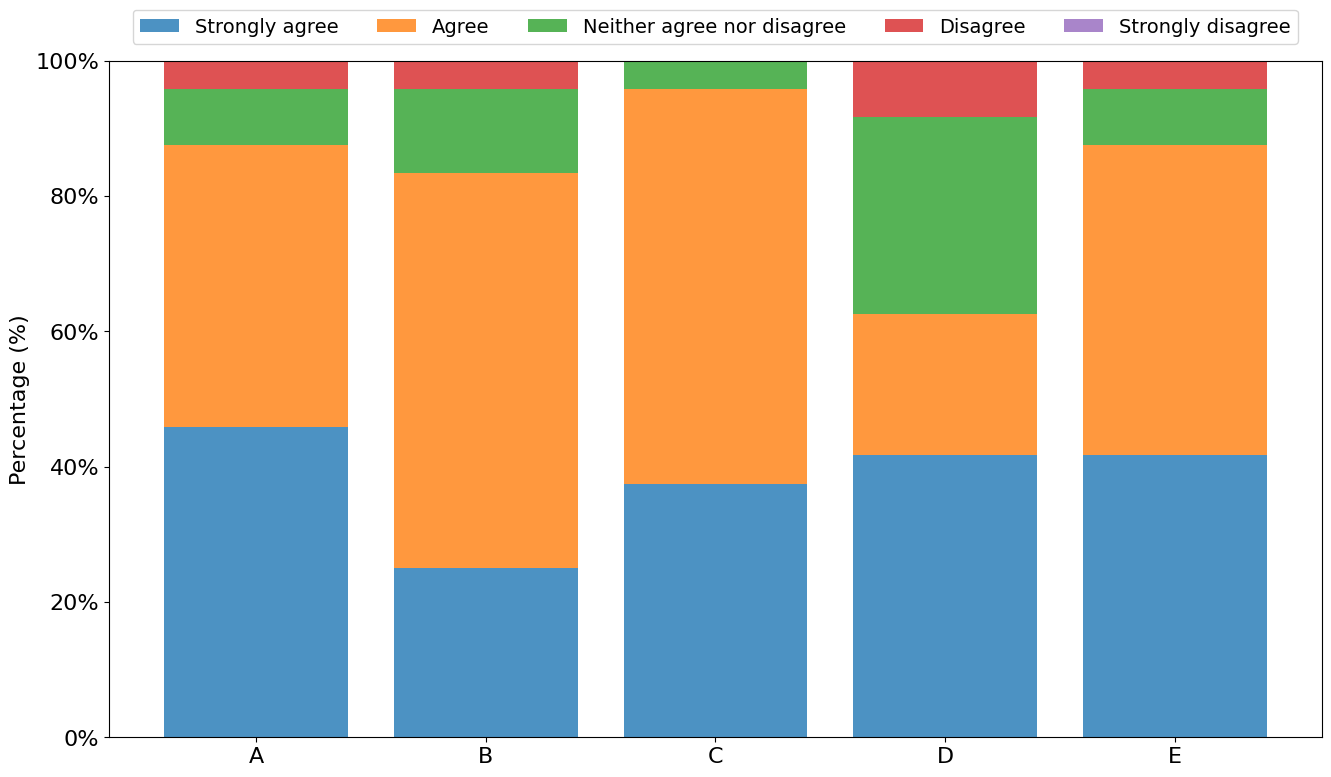
\includegraphics[width=\columnwidth,keepaspectratio]{likert.png}
    \caption{The stacked bar chart shows the user study participant responses of Likert Scale questions.}
    \label{fig:likert}
\end{figure}
}

The qualitative results clearly support our hypothesis H1 that rivers generally increase the legibility of cartograms.

\section{Limitations and Future Work}
\label{sec:{Limitations and Future Work}}

In this section, we discuss some limitations of our work and future research directions.
Because this is a new concept, it opens the door for many future research directions.

\subsection{Color map choice}

The first limitation is the color map that we use to depict the data in our cartograms.
    We use D3's built-in interpolateRdYlGn color map, a diverging color scheme of red, yellow, and green.
    However, we believe that the choice of color map can have a significant impact on the legibility of cartograms.
    In the user study, we carefully avoid extreme values where the location or color of the CCG makes it easier to locate the target.
    See \Cref{fig:extreme} for an example. We plan to explore the impact of different color maps on the legibility of cartograms in future work.

    {
        \begin{figure}[tb!]
            \centering
            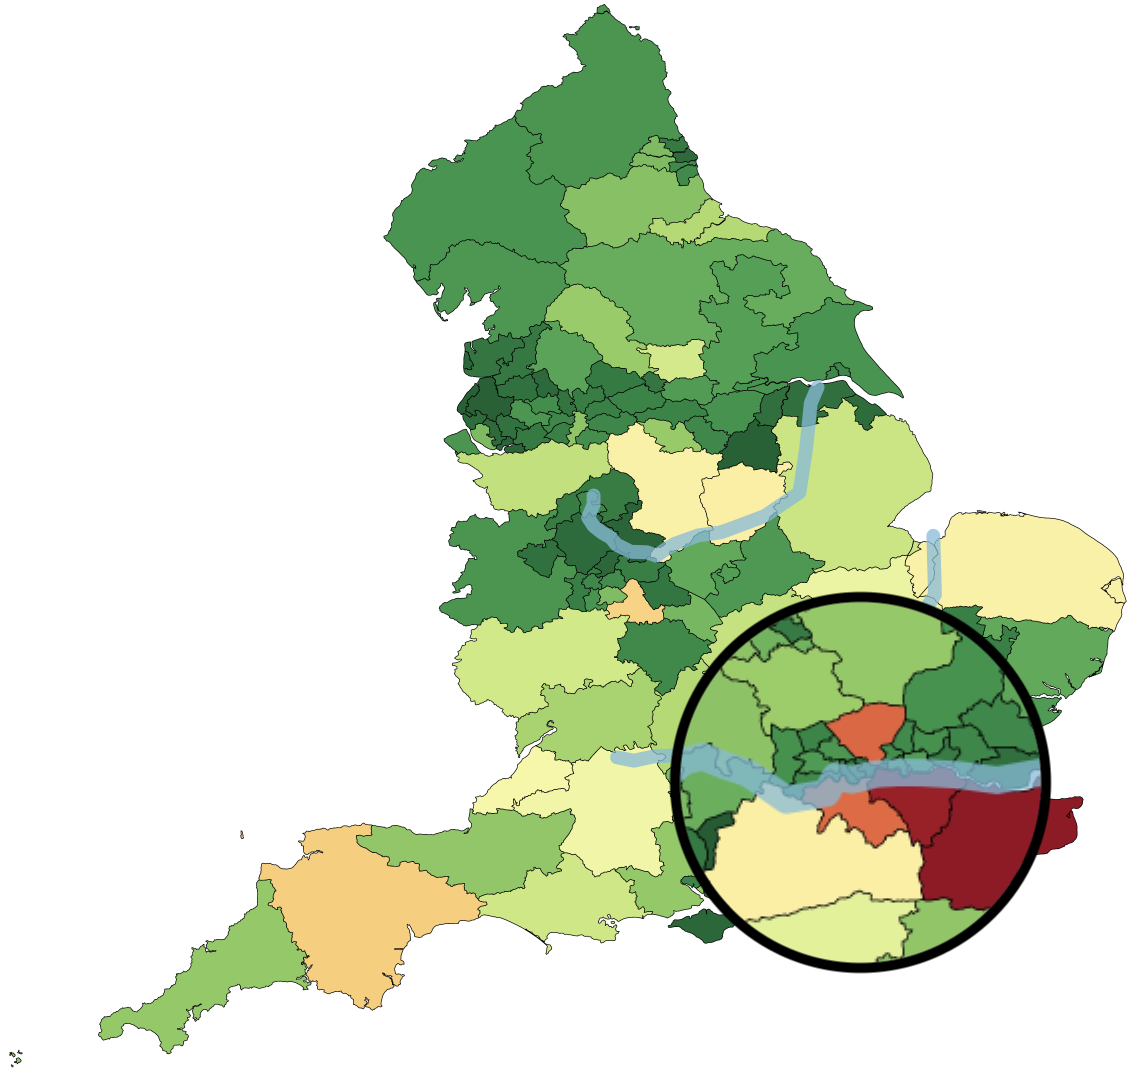
\includegraphics[width=0.8\columnwidth,keepaspectratio]{extreme.png}
            \caption{Due to color and relative location, we believe the CCGs in the black circle are easier to locate.}
            \label{fig:extreme}
        \end{figure}
    }

\subsection{Overlap removal algorithm choice}

Another limitation is the algorithm (FNOR) we use.
We believe that developing a new algorithm with built-in constraint support can significantly reduce the time required to generate cartograms with rivers.
Currently, the runtime of our layout algorithm is approximately 30 milliseconds for each iteration. When the quantity of nodes and features increases, generating the optimal layout demands several hundred iterations.

\subsection{Generalizability}

Future work also includes generalizations and extensions of the algorithm, e.g., the use of other features in the cartogram layout such as additional rivers, major highways, lakes, and coastlines, etc.
We also consider whether increasing the length of the rivers as the size of the nodes increases would be a useful option.
We would like to explore the case of river-river intersections (or confluence) and testing out more geographies such as the U.S.
and Europe, which have more complex rivers.
We also considered the idea of deforming the rivers as part of the layout algorithm, however, this idea is open to future work.

\subsection{Improved User Study}

Due to pandemic restrictions, the user study did not take place in a controlled environment.
In the future, we aim to execute a more controlled laboratory study, ensuring a controlled environment and standardized hardware for participants.


\section{Conclusions}\label{sec:{Conclusions}}

In this paper, we present a novel hybrid layout approach to generate non-contiguous cartograms with rivers.
We first propose a new algorithm to generate cartograms with rivers, and then we present a prototype to support the exploration of cartograms with rivers.
We evaluate our approach with a preliminary user study, and the results support our hypotheses: the introduction of rivers improves the legibility and recognizability of cartograms, although a deeper analysis is necessary to reach more confident conclusions.
We also discuss the limitations of our work and future research directions.



\section{Acknowledgements}
This work is funded by the grant EP/S010238/2 from the Engineering and Physical Sciences Research Council (EPSRC). EPSRC is a British Research Council that provides government funding for grants to undertake research and postgraduate degrees in engineering and the physical sciences.



\bibliographystyle{elsarticle-num-names}
\bibliography{references}
\cleardoublepage

\appendix

\section{Obtaining Shapefile}
\label{obtaining-shapefile}
\begin{lstlisting}[caption={The query that downloads the shapefile of River Thames from OpenStreetMap via the Overpass Turbo API.}, label={overpass},captionpos=b]
    relation(2263653);>>;
    // River Great Ouse: 2798097
    // River Trent: 2863468
    out skel;
\end{lstlisting}

\section{Pre-processing Shapefiles}
\label{app:pre-processing}
Shapefiles from different sources are likely to be incompatible.
In our case, the NHS CCG shapefile is incompatible with the river shapefiles.
The major reason for the incompatibility is the coordinate reference system (CRS).
The CRS of the CCG shapefile is EPSG:27700 (OSGB36 - British National Grid).
The CRS of the river shapefiles is EPSG:4326 (WGS84 - World Geodetic System).
Here, we provide some pre-processing steps using QGIS (version: 3.26.0-Buenos Aires) \cite{qgisWelcome} to handle the incompatibility and reduce shapefile size to improve performance.

\subsection{Import Shapefiles into QGIS}
We first load all three river shapefiles into QGIS \Cref{fig:import_rivers}, followed by the CCG shapefile \Cref{fig:import_ccgs}.

{
\begin{figure}[H]
    \centering
    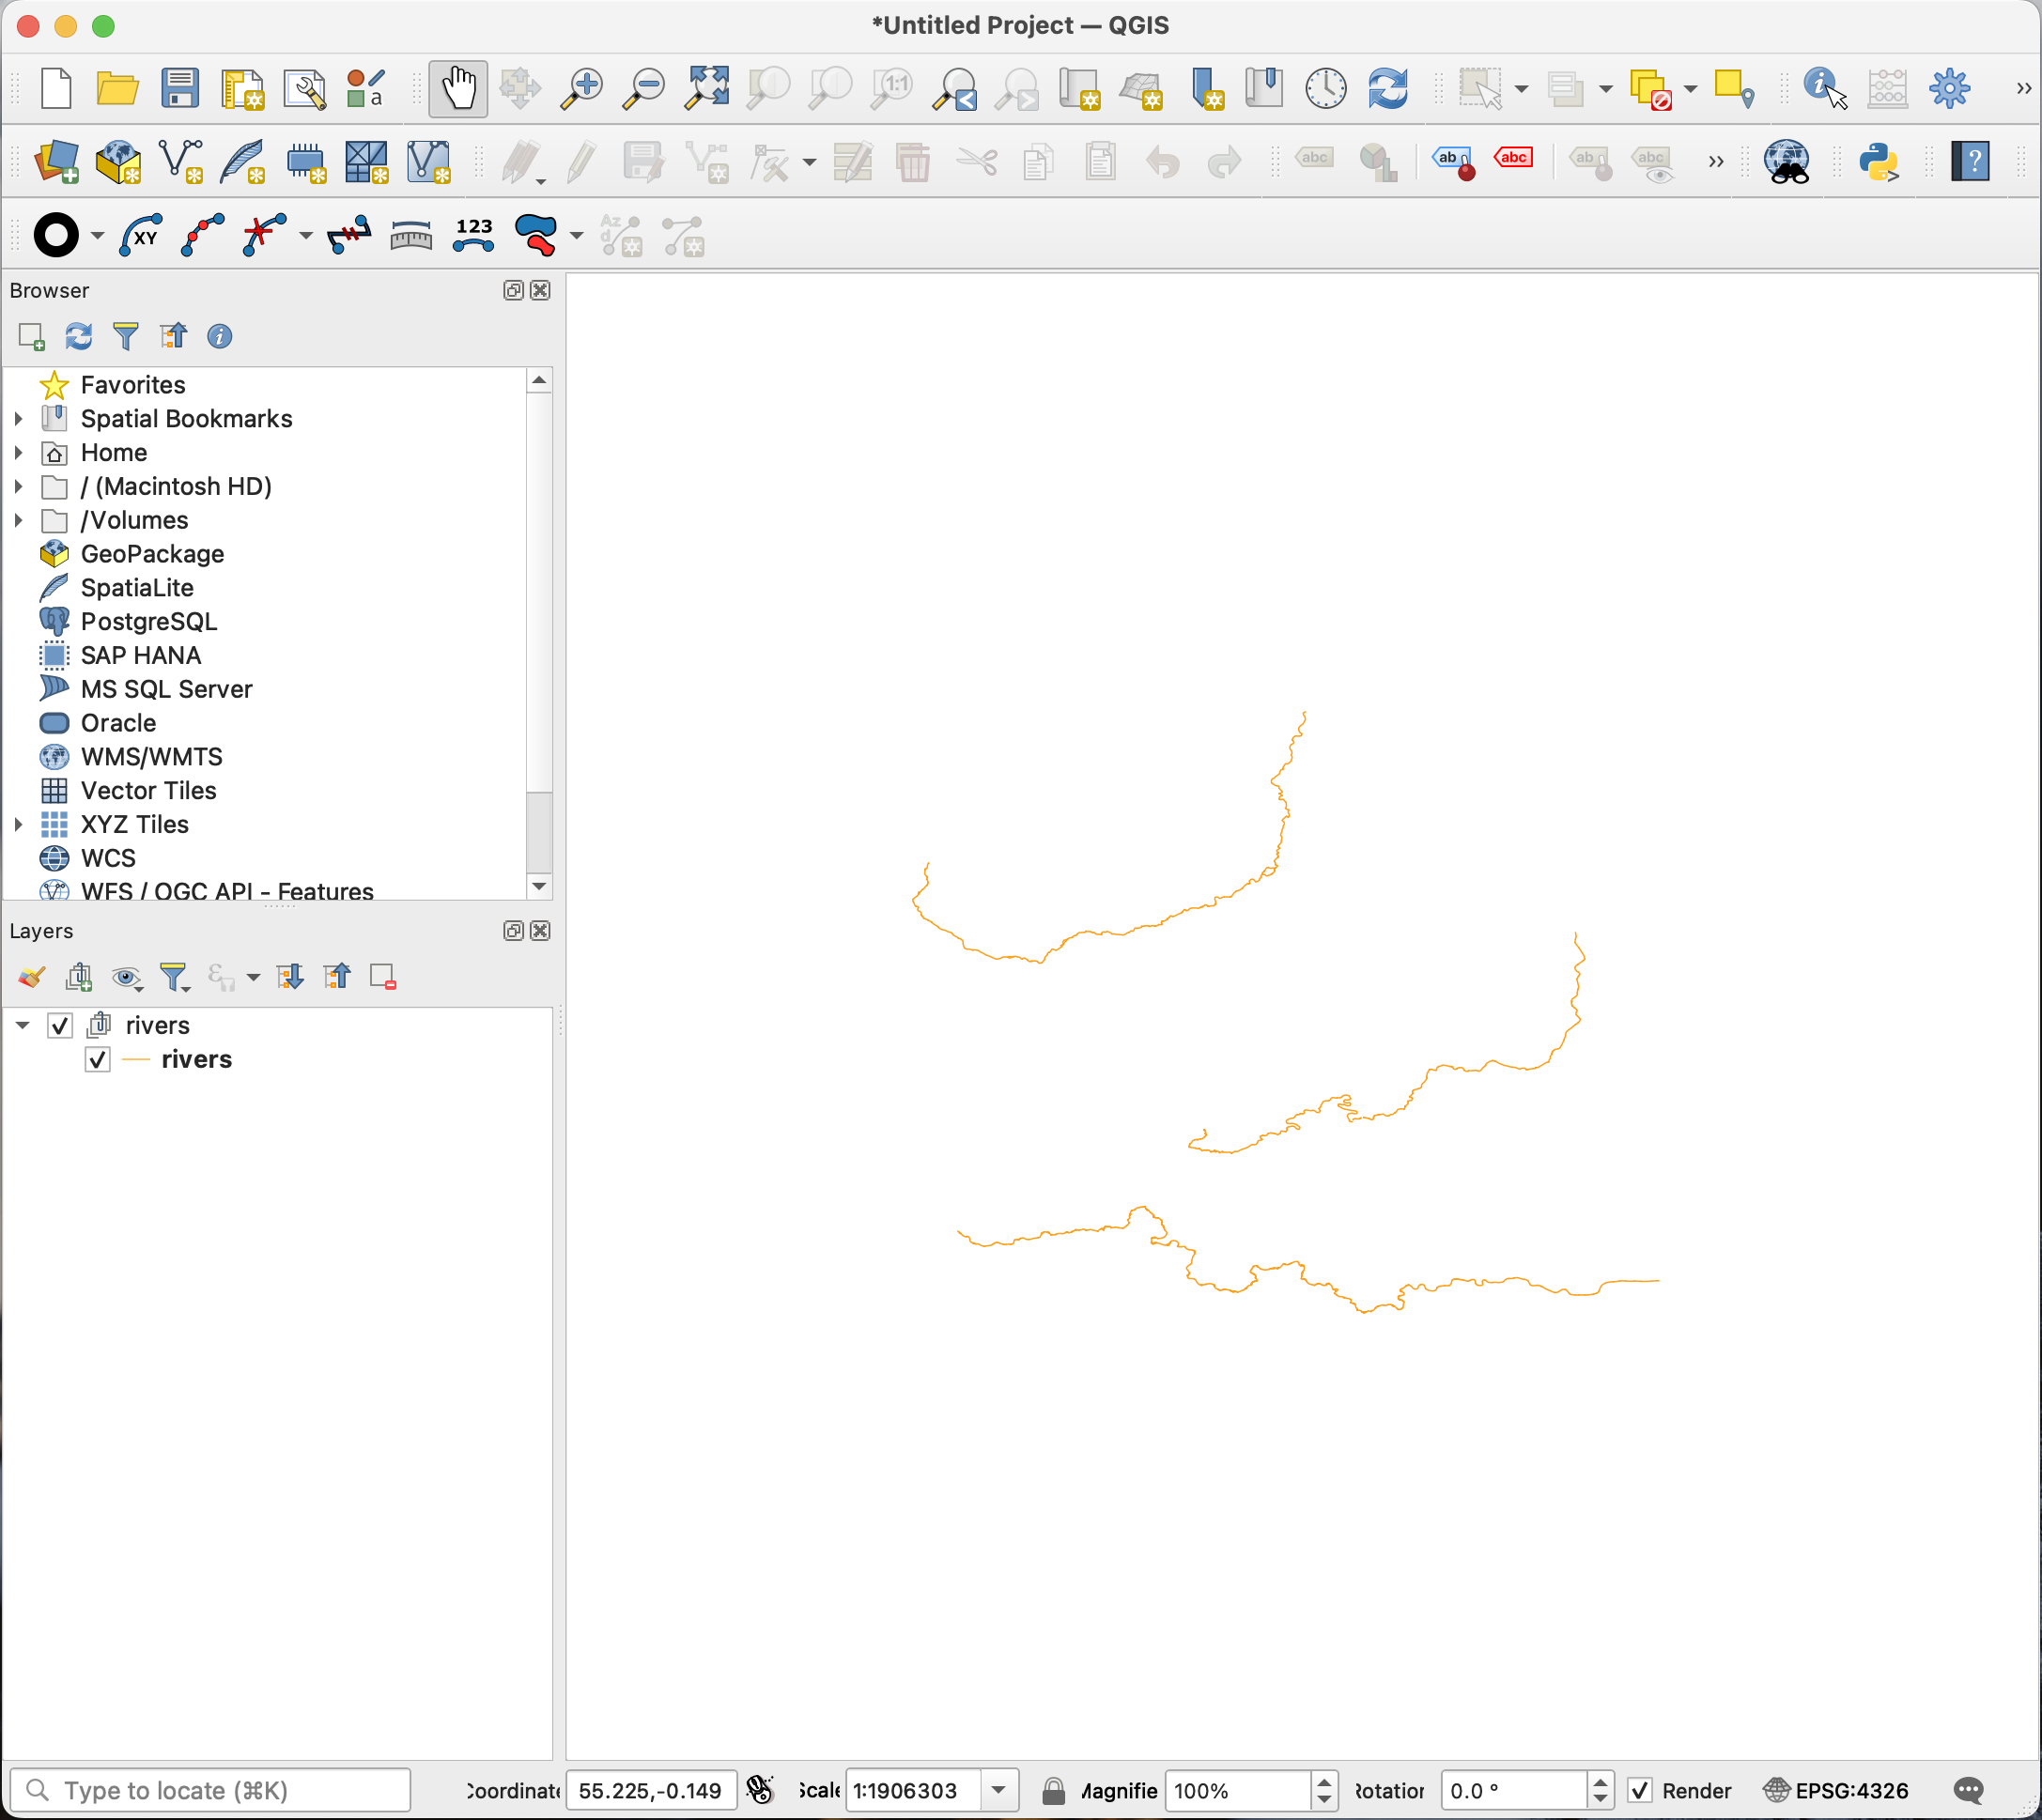
\includegraphics[width=\columnwidth]{import_rivers.png}
    \caption{QGIS interface, with River Trent, River Great Ouse, and River Thames (from top to bottom) imported.}
    \label{fig:import_rivers}
\end{figure}

\begin{figure}[H]
    \centering
    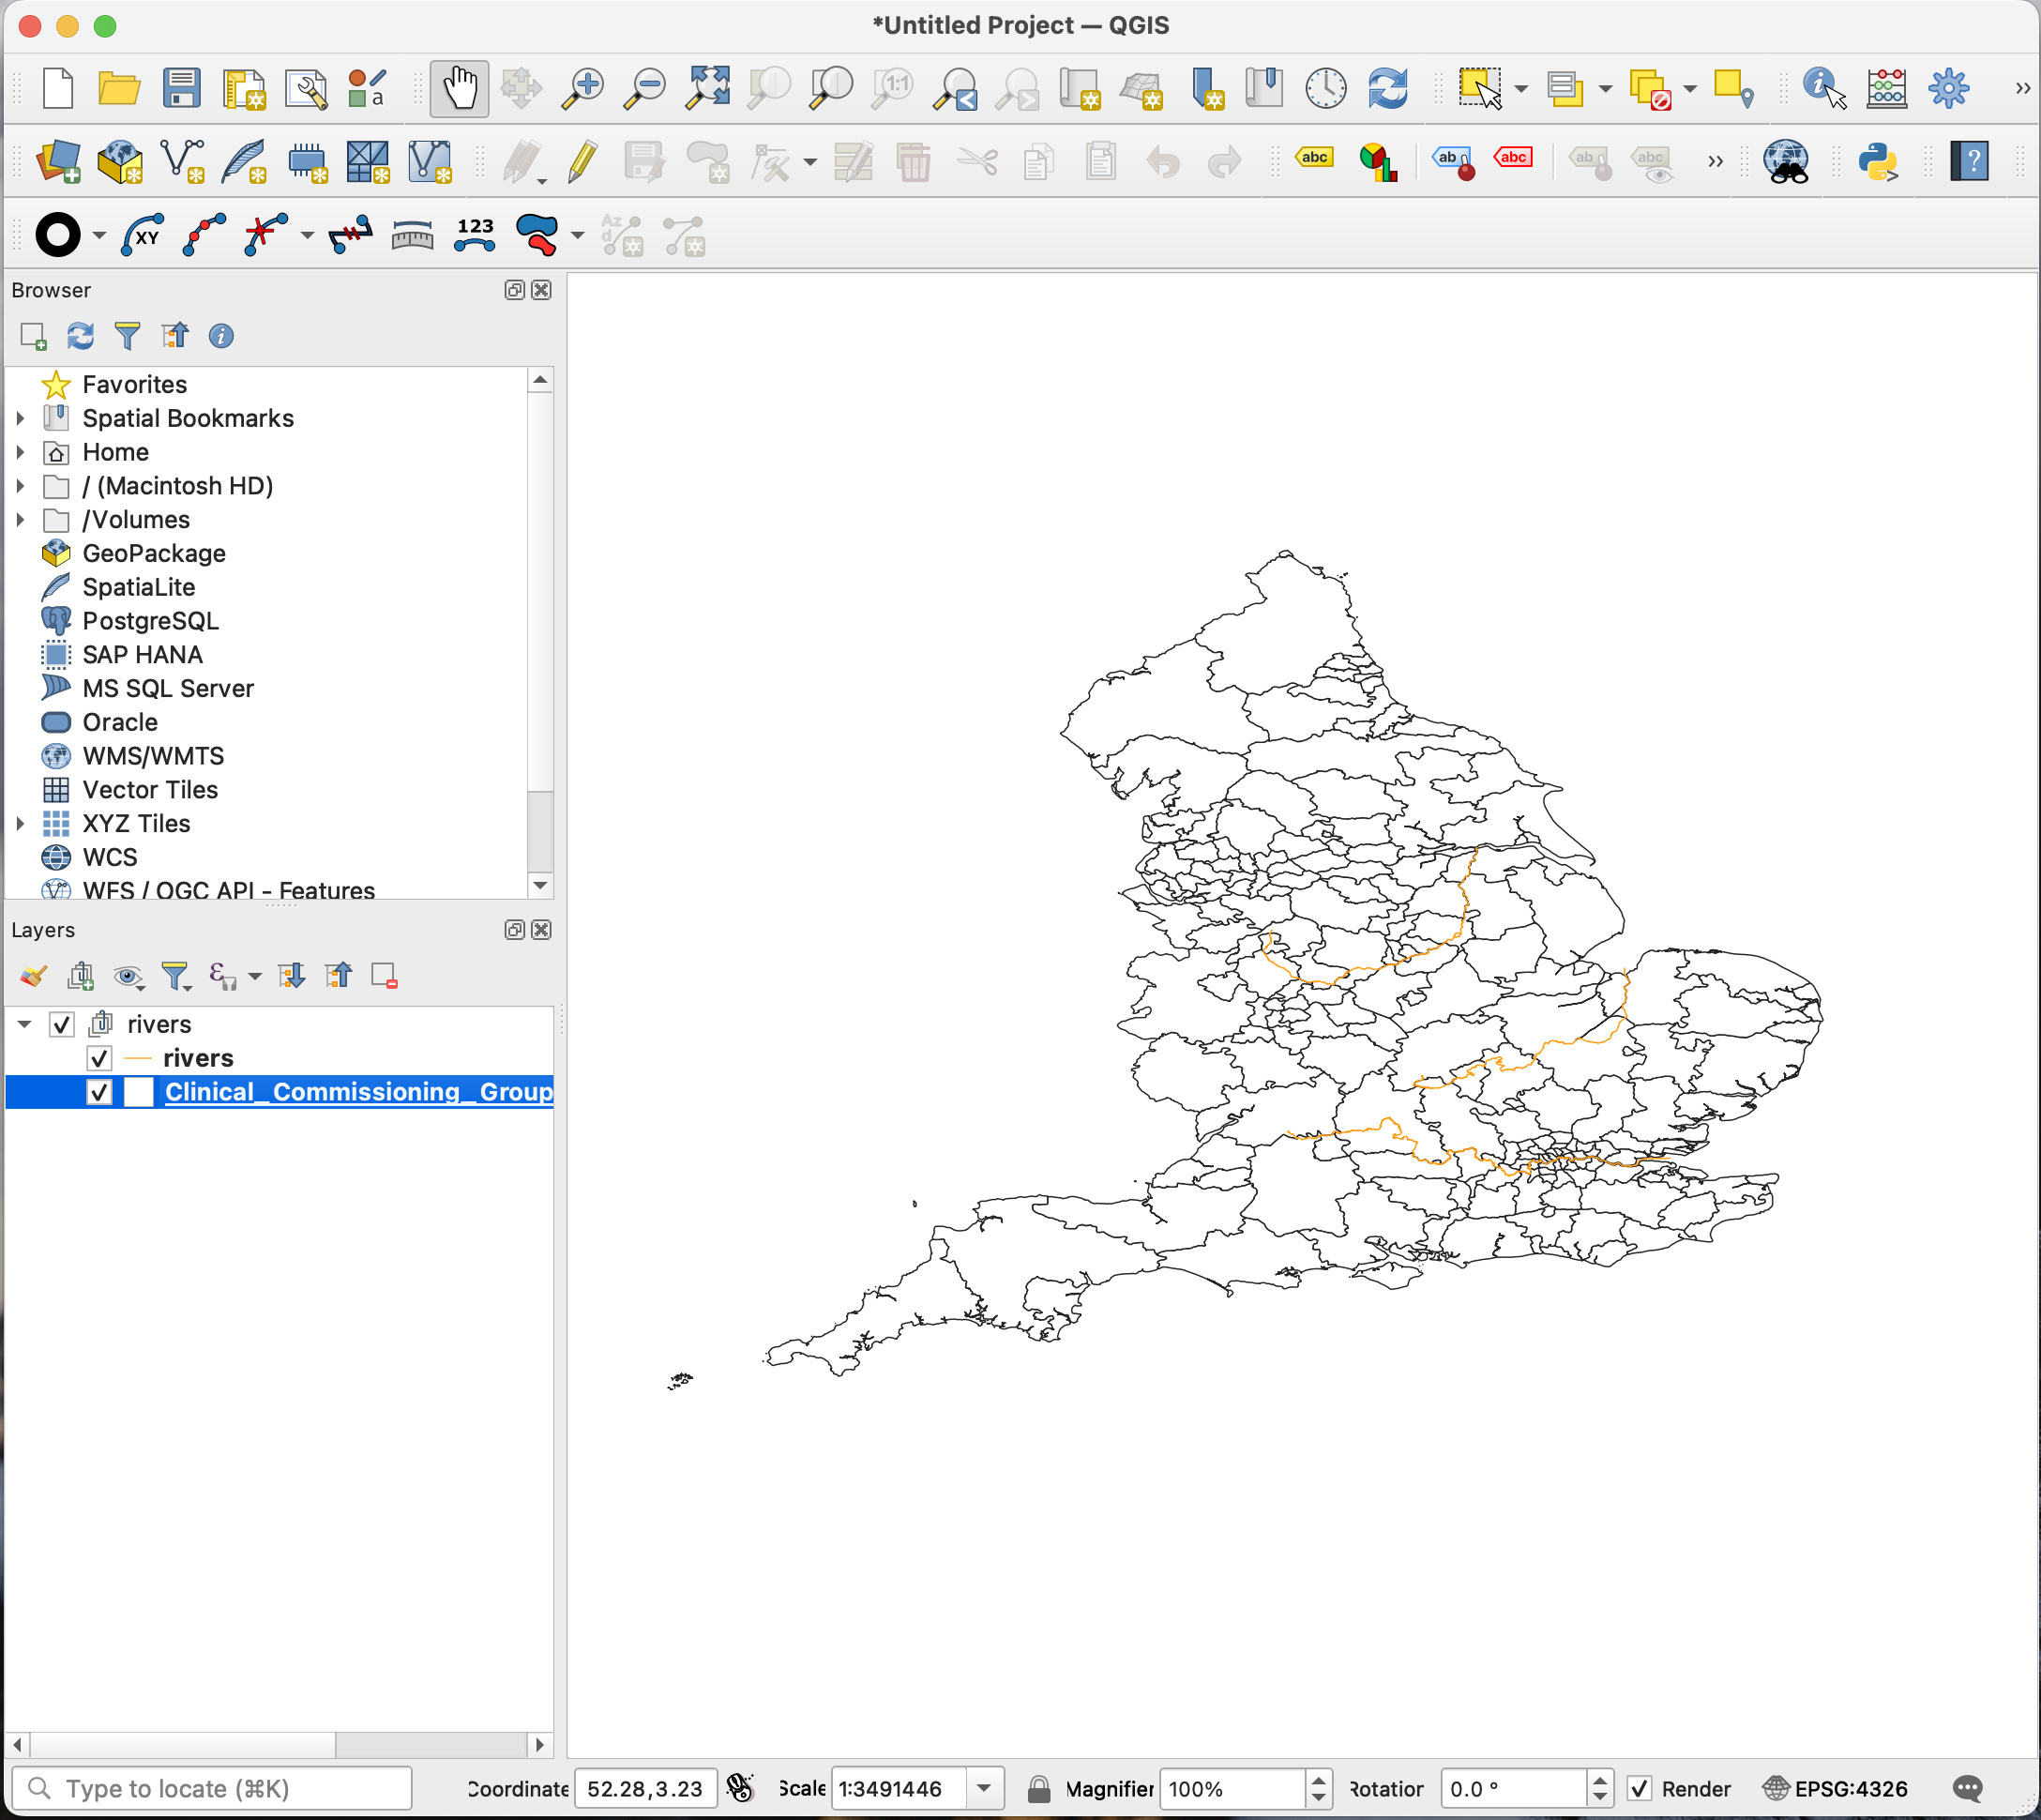
\includegraphics[width=\columnwidth]{import_ccgs.png}
    \caption{QGIS interface, with all NHS CCGs imported.}
    \label{fig:import_ccgs}
\end{figure}

\begin{figure}[H]
    \centering
    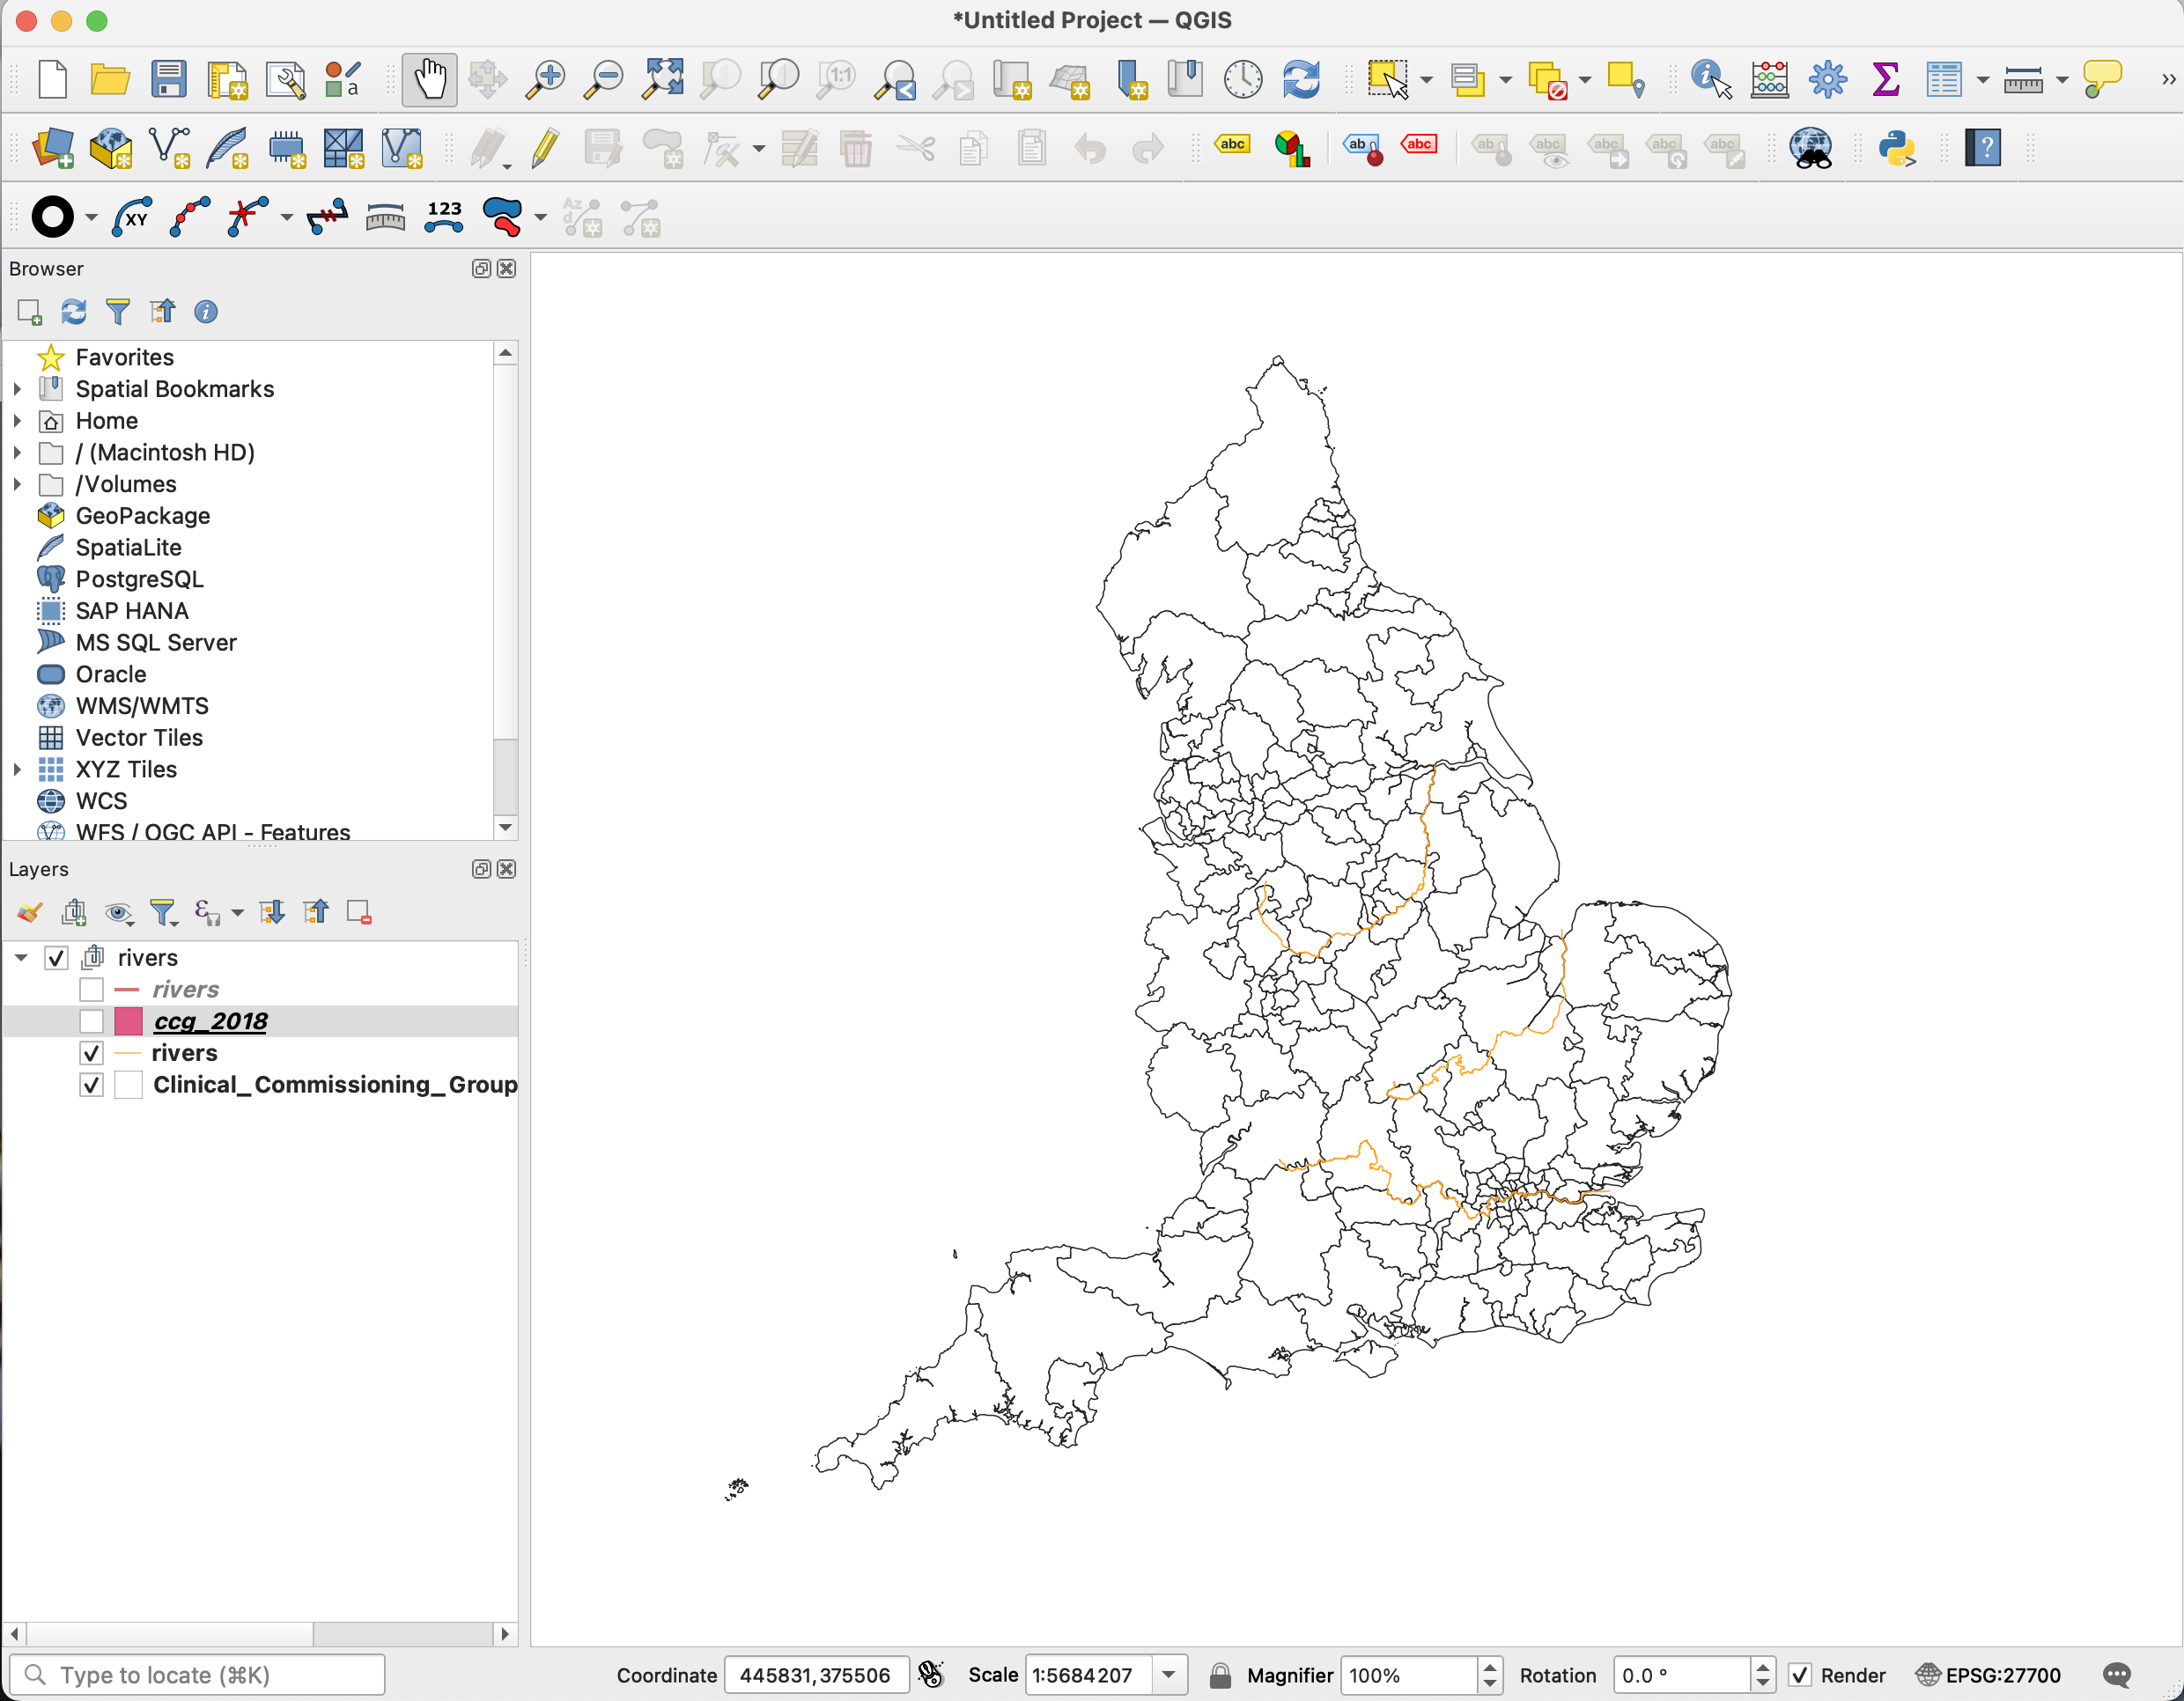
\includegraphics[width=\columnwidth]{unify_crs.png}
    \caption{QGIS interface, showing the unified CRS (OSGB36) for both layers.}
    \label{fig:unify_crs}
\end{figure}
}

\subsection{Export Shapefiles in GeoJSON and Unify the Coordinate Reference System (CRS)}

We then use QGIS to unify the CRS, and export both layers in GeoJSON format.
See \Cref{fig:export_rivers} and \Cref{fig:export_ccgs}.
The unified layer is shown in \Cref{fig:unify_crs}.

{
\begin{figure}[H]
    \centering
    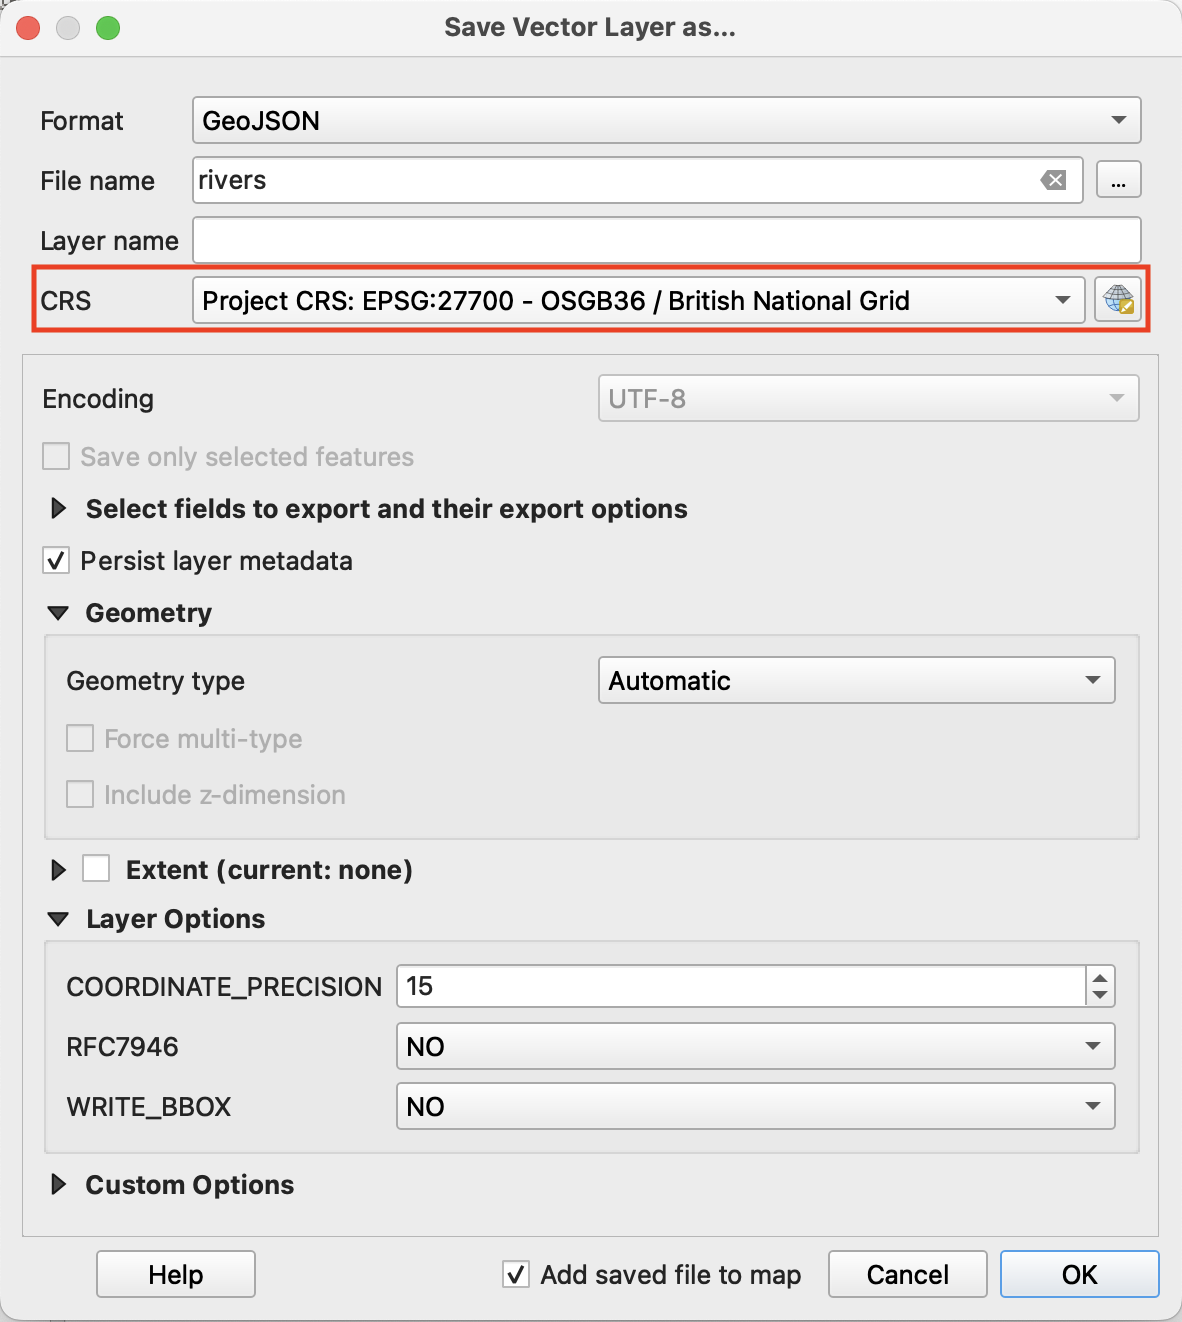
\includegraphics[width=\columnwidth]{export_rivers.png}
    \caption{QGIS interface, exporting all rivers using the OSGB36 CRS in GeoJSON.}
    \label{fig:export_rivers}
\end{figure}

\begin{figure}[H]
    \centering
    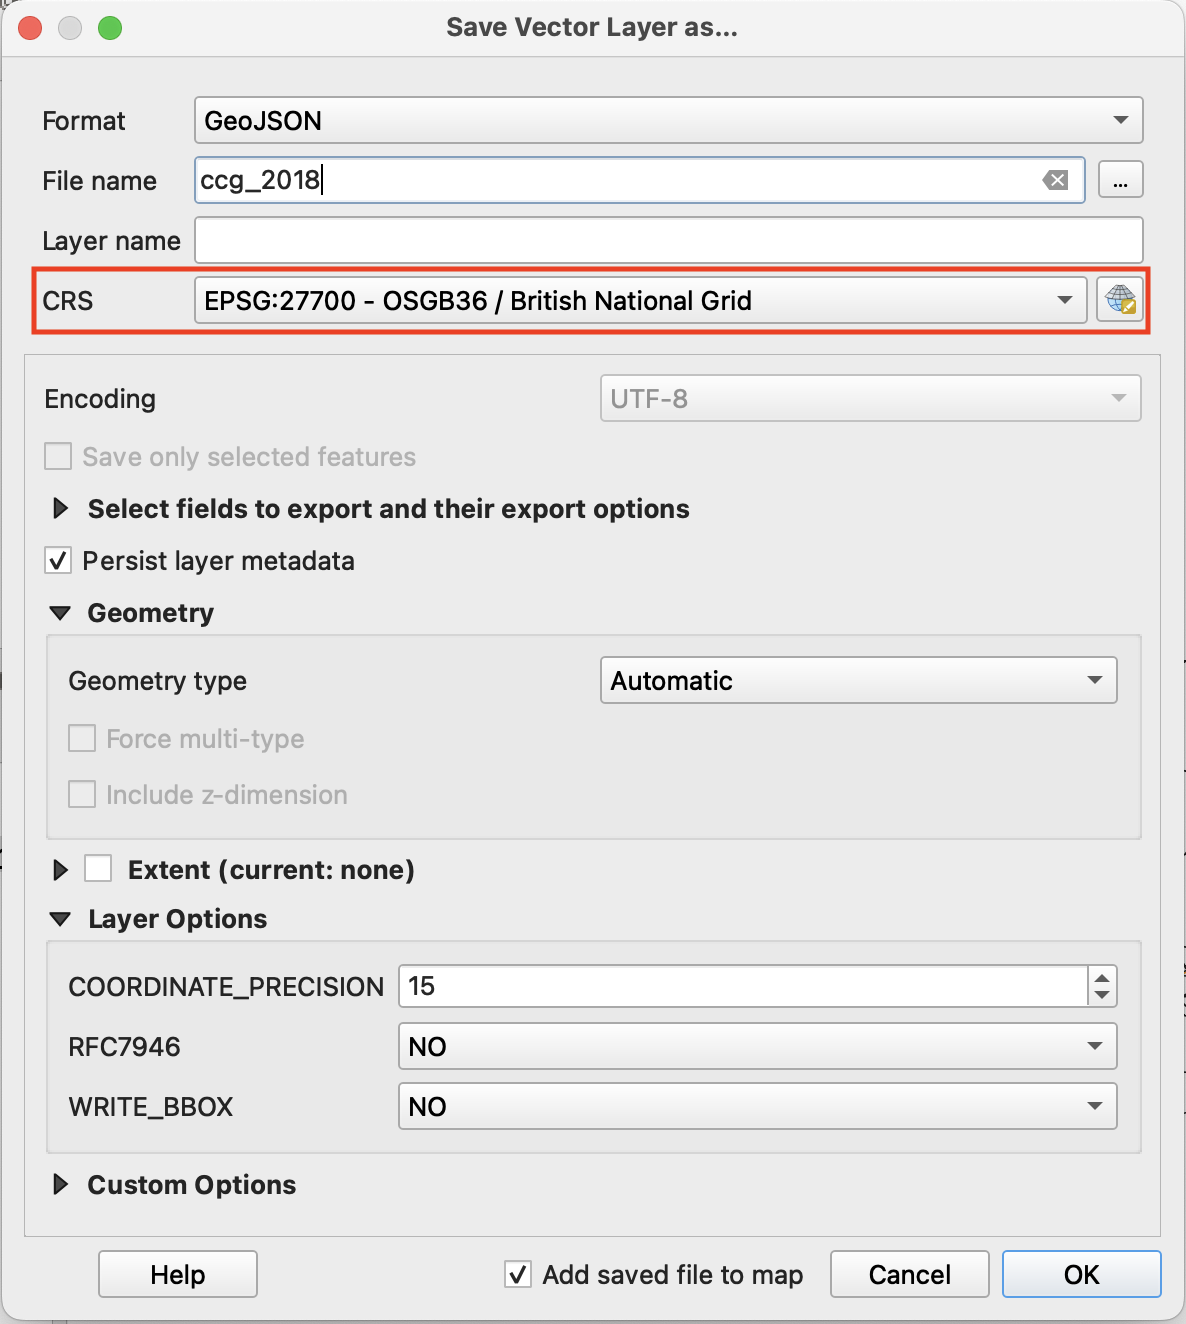
\includegraphics[width=\columnwidth]{export_ccgs.png}
    \caption{QGIS interface, exporting all NHS CCGs using the OSGB36 CRS in GeoJSON.}
    \label{fig:export_ccgs}
\end{figure}

}

\subsection{Merge Shapefiles and Reduce File Size}

We then merge two layers into one layer, and export it in the TopoJSON format using Mapshaper \cite{blochMapshaper}.
Mapshaper also supports the simplification of GeoJSON shapefiles.
See \Cref{fig:export_topojson}.

{
\begin{figure}[H]
    \centering
    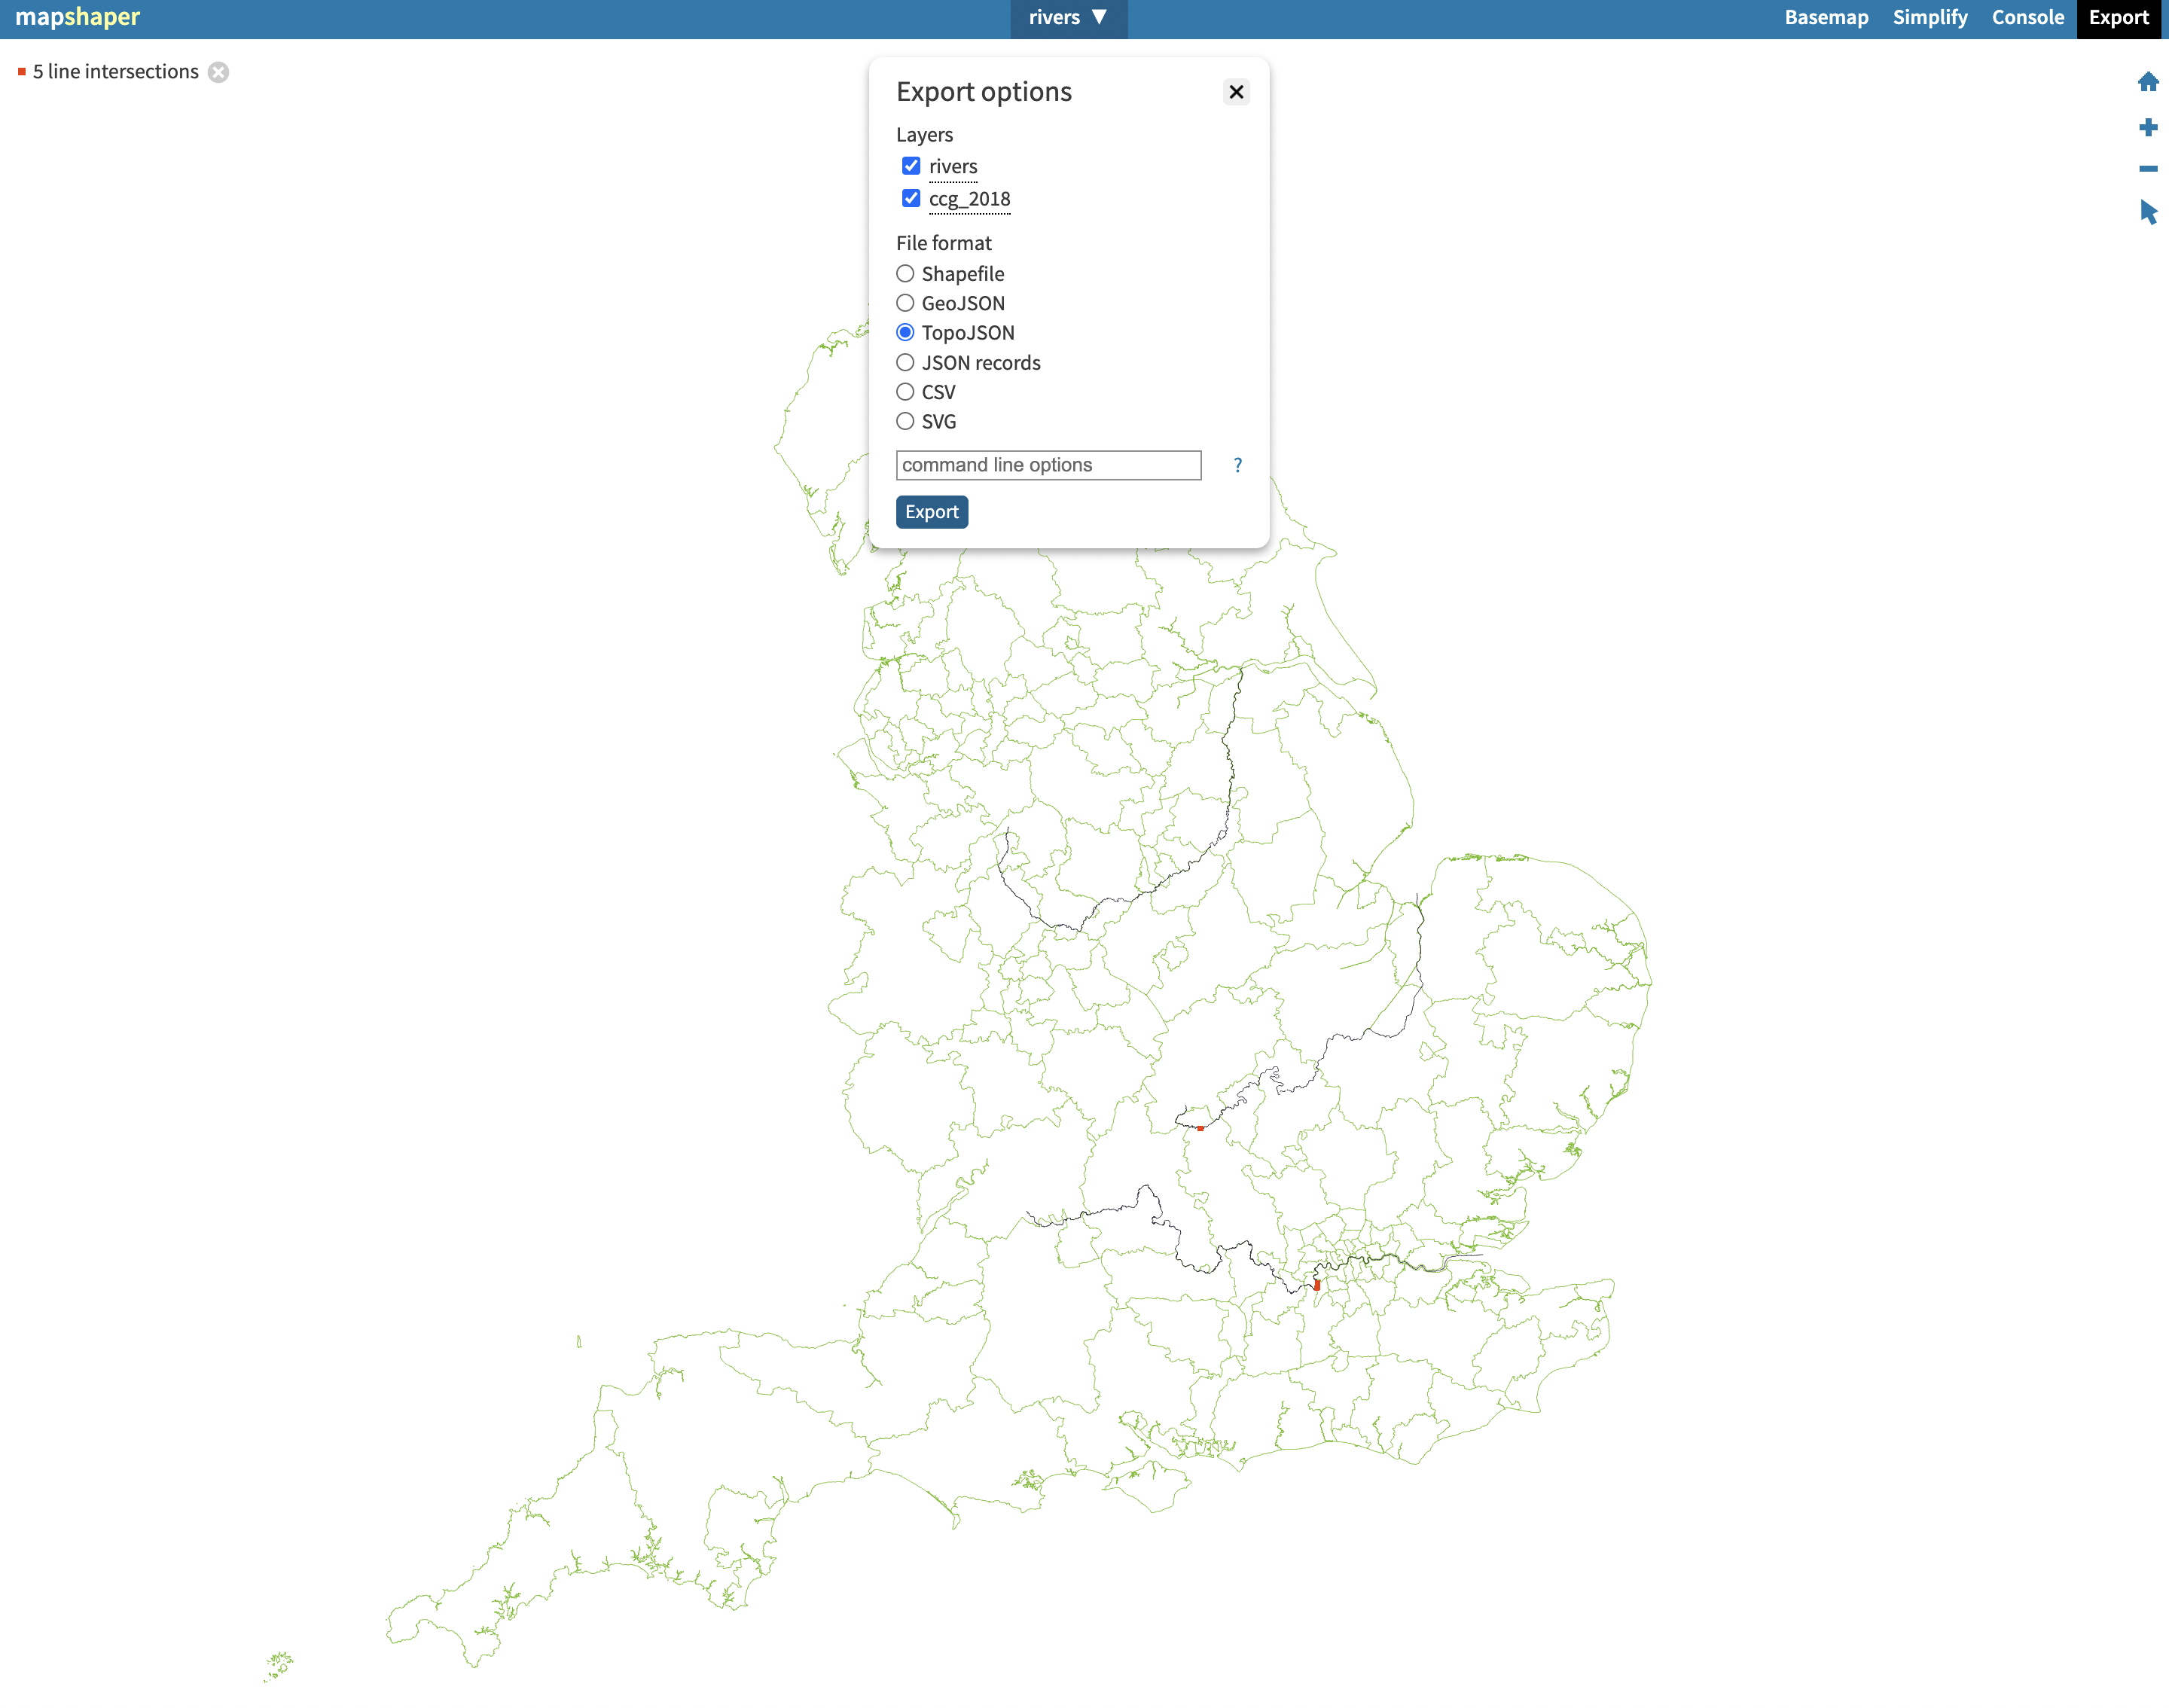
\includegraphics[width=\columnwidth]{export_topojson.png}
    \caption{Mapshaper interface, merging all rivers with NHS CCGs into one layer, and export the merged layer in TopoJSON.}
    \label{fig:export_topojson}
\end{figure}
}

\subsection{Pre-processing Result}

\Cref{table:pre-processing_result} shows the preprocessing result.
The reduction in file size is significant and greatly reduces the initialization time of our implementation.

    {
        \renewcommand{\arraystretch}{1.5}
        \begin{table}[H]
            \centering
            \resizebox{\columnwidth}{!}{
                \begin{tabulary}{\columnwidth}{|*{4}{l|}}
                    \hhline{~|*{3}{-}}
                    \multicolumn{1}{c|}{\textbf{Shapefile}} &
                    \cellcolor{Mycolor2}\textbf{Original} &
                    \cellcolor{Mycolor2}\textbf{GeoJSON} &
                    \cellcolor{Mycolor2}\textbf{TopoJSON} \\
                    \hline
                    Rivers & 2.0 MB (GeoJSON) & 1.4 MB & -  \\
                    \hline
                    NHS CCGs & 46.6 MB (.shp, Esri vector shapefile) & 140.2 MB & -  \\
                    \hline
                    Merged & - & - & 16.3 MB \\
                    \hline
                \end{tabulary}
            }
            \caption{The file size is reduced by 88.5\% from the original size.}
            \label{table:pre-processing_result}
        \end{table}
    }

% \clearpage
\section{Procedure: DeriveParallelEdge}
% \begin{noindent}

    \begin{algorithm}[H]
        \caption{Procedure to derive an edge, $ \EdgeParallel $, that is parallel to $ \Edge $ with a distance of $ \Distance $.}\label{alg:derive corridor edge}

        \textbf{Input:} \\
        $ \Edge \gets $ the edge used to derive the parallel edge $ \EdgeParallel $ \\
        $ \Distance \gets $ the shortest distance between $ \Edge $ and $ \EdgeParallel $ \\

        \textbf{Output:} \\
        An edge, $ \EdgeParallel $, that is parallel to $ \Edge $ with a distance of $ \Distance $.
\\

        \textbf{Local variables:} \\
        $ \dx, \dy \gets $ the differences in $ x, y $ for $ \EdgeStart $ and $ \EdgeEnd $ \\
        $ \Scale \gets $ the scale of $ \frac{\Distance}{\sqrt{\dx^2 + \dy^2}} $ \\

        \begin{algorithmic}[1]
            \Procedure{DeriveParallelEdge}{$ \Edge $, $ \Distance $}
                \State $ \dx \gets \EdgeStart.x - \EdgeEnd.x $

                \State $ \dy \gets \EdgeStart.y - \EdgeEnd.y $

                \State $ \Scale \gets \frac{\Distance}{\sqrt{\dx^2 + \dy^2}} $

                \State $ \EdgeParallel.start.x \gets \Scale \cdot (-\dy) + \EdgeStart.x $

                \State $ \EdgeParallel.start.y \gets \Scale \cdot \dx + \EdgeStart.y $

                \State $ \EdgeParallel.end.x \gets \Scale \cdot (-\dy) + \EdgeEnd.x $

                \State $ \EdgeParallel.end.y \gets \Scale \cdot \dx + \EdgeEnd.y $

            \State \Return{$ \EdgeParallel $}

            \EndProcedure

        \end{algorithmic}
    \end{algorithm}
%\end{noindent}


\section{Procedure: TranslateNode}

\begin{algorithm}[H]
    \caption{Procedure to translate node positions.}\label{alg:TranslateNode}

    \textbf{Input:} \\
    $ \nodeList \gets $ a list of $ \node $ representing regions \\

    \textbf{Output:} \\
    $ \nodeTopologicalError \gets $ the number of nodes crossing the river in the input \\

    \textbf{Global variables:} \\
    $ \stalemateMax \gets $ the maximum number of iterations indicating a stalemate \\

    \textbf{Local variables:} \\
    $ \node \gets $ a node is an object with the following properties: \\
    \-\hspace{1em} $ \node.x, \node.y, $ or $ \node(x,y) \gets $ the x and y coordinates of $ \node $ \\
    \-\hspace{1em} $ \nodeCross \gets $ the number of times that $ \node $ crosses a river  \\
    \-\hspace{1em} $ \nodePrevious \gets $ the previous position of $ \node $ \\
    \-\hspace{1em} $ \nodeFNOR \gets $ the translated position of $ \node $ \\

    \begin{algorithmic}[1]
        \Procedure{TranslateNode}{$ \nodeList $}
        \State $ \nodeTopologicalError \gets 0 $
        \ForEach {$ \node \in \nodeList $}

        \If {$ \node(x,y) \neq \nodeFNOR(x,y) $}

        \State $ \node(x,y) \gets \nodeFNOR(x,y) $

        \If{ \Call{TestIntersection}{$ \nodeFNORLine $} $ = True $}
        \State $ \nodeCross ++ $
        \State $ \nodeTopologicalError ++ $

        \If{$ \nodeCross < \stalemateMax $}
        \State \hskip-2em \Comment{Translate back to previous position}
        \State $ \node(x,y) \gets \nodePrevious(x,y) $

        \Else

        \State \Call{ProcessStalemate}{$ \node, \nodeFNOR $}
        \State $ \nodeCross \gets 0 $ \Comment{Reset counter}

        \EndIf

        \EndIf

        \EndIf

        \EndFor
        \State \Return{$ \nodeTopologicalError $}
        \EndProcedure
    \end{algorithmic}
\end{algorithm}
\vfill\eject

\section{Procedure: UpdateLayout}

\begin{algorithm}[H]
    \caption{Procedure to adjust river positions, remove node overlap and prevent nodes from crossing rivers.
        See \Cref{sec:main}.}\label{alg:UpdateLayout}
    \textbf{Global variables:} \\
    $ \nodeList \gets $ a list of $ \node $ representing regions with the following properties: \\
    \-\hspace{1em}  $\nodeListCross \gets $ the number of $ \node $ in $ \nodeList $ that crosses a river \\

    $ \nodeSize \gets $ the initial size of all nodes \\
    $ \nodeCartographicError \gets $ the average cartographic error of all nodes \\
    $ \nodeCartographicErrorMax \gets $ the maximum cartographic error of all nodes \\
    $ \stalemateMax \gets $ the maximum number of iterations indicating a stalemate \\

    \textbf{Local variables:} \\
    $ \node \gets $ a node is an object with the following properties: \\
    \-\hspace{1em} $ \node.x, \node.y, $ or $ \node(x,y) \gets $ the x and y coordinates of $ \node $ \\
    \-\hspace{1em} $ \nodeCross \gets $ the number of times that $ \node $ crosses a river \\
    \-\hspace{1em} $ \nodePrevious \gets $ the previous position of $ \node $ \\
    \-\hspace{1em} $ \nodeFNOR \gets $ the translated position of $ \node $ \\

    \begin{algorithmic}[1]
        \Procedure{UpdateLayout}{}

        \State $ \nodeSize \gets 1 $
        \While{$ \nodeCartographicError < \nodeCartographicErrorMax $}
        \State $ \nodeListCross \gets 1 $ \Comment{Trigger the while loop}
        \While{$ \nodeListCross > 0 $}

        \State $ \nodeListCross \gets 0 $
        \State $ \nodeList \gets $ RemoveOverlap ($ \nodeList $)
        \State \Call{TranslateRiver}{$ \nodeList $}
        \State $\nodeListCross \gets $ \Call{TranslateNode}{$ \nodeList $}

        \EndWhile

        \State $ \nodeSize ++ $

        \EndWhile

        \EndProcedure
    \end{algorithmic}
\end{algorithm}
\vfill\eject

\section{Procedure: TranslateRiver}

\begin{algorithm}[H]
    \caption{Procedure to translate rivers.}\label{alg:TranslateRiver}
    \textbf{Input:} \\
    $ \nodeList \gets $ a list of $ \node $ representing regions \\

    \textbf{Local variables:} \\
    $ \riverList \gets $ a list of $ \river $ representing river features \\
    $ \node \gets $ a node is an object with the following properties: \\
    \-\hspace{1em} $ \node.x, \node.y, $ or $ \node(x,y) \gets $ the x and y coordinates of $ \node $ \\
    \-\hspace{1em} $ \nodePrevious \gets $ the previous position of $ \node $ \\
    \-\hspace{1em} $ \nodeFNOR \gets $ the translated position of $ \node $ \\
    $ \nodeTopologicalError \gets $ the number of nodes intersecting $ \river $  \\

    \begin{algorithmic}[1]
        \Procedure{TranslateRiver}{$ \nodeList $}
        \ForEach {$ \river \in \riverList $}
        \State $ \nodeTopologicalError \gets 0 $
        \State $ \riverVector \gets (0,0) $ \Comment{Hold the sum of vectors $ \nodeVectorCT $}
        \ForEach {$ \node \in \nodeList $}

        \If {$ \node(x,y) \neq \nodeFNOR(x,y) $}
        \If{ \Call{TestIntersection}{$ \nodeFNORLine $, $ \river $} $ = True $}
        \State $ \riverVector \gets \riverVector + \nodeVectorCT$
        \State $ \nodeTopologicalError ++ $
        \EndIf

        \EndIf

        \EndFor

        \State Translate river $ \river $ by the average vector $ \frac{\riverVector}{\nodeTopologicalError} $
        \EndFor

        \EndProcedure
    \end{algorithmic}
\end{algorithm}


\section{Procedure: DerivePoint}
% \begin{noindent}

    \begin{algorithm}[H]
        \caption{Procedure to derive a point based an edge and a distance.}\label{alg:derive corridor point}
        \textbf{Input:} \\
        $ \Edge \gets $ the edge used to derive the new point \\
        $ \Distance \gets $ the distance between $ \PointP $ and $ \EdgeStart $ \\

        \textbf{Output:} \\
        A point, $ \PointP $, that is distance $ \Distance $ away from $ \EdgeStart $.
\\
    
        \textbf{Local variables:} \\
        $ \dx, \dy \gets $ the differences in $ x, y $ for $ \EdgeStart $ and $ \EdgeEnd $ \\
    
        \begin{algorithmic}[1]
            \Procedure{DerivePoint}{$ \Edge $, $ \Distance $}
                \State $ \dx \gets \EdgeStart.x - \EdgeEnd.x $
    
                \State $ \dy \gets \EdgeStart.y - \EdgeEnd.y $
    
                \State $ \PointP.x \gets \frac{\dx}{\sqrt{\dx^2 + \dy^2}} \cdot \Distance $
    
                \State $ \PointP.y \gets \frac{\dy}{\sqrt{\dx^2 + \dy^2}} \cdot \Distance $
    
            \State \Return{$ \PointP $}
    
            \EndProcedure
    
        \end{algorithmic}
    \end{algorithm}
    
%\end{noindent}
% \vfill\eject


\section{Procedure: ProcessStalemate}

% \begin{noindent}

    \begin{algorithm}[H]
        \caption{Procedure to derive a corridor to resolve stalemate.
We use an SVG canvas, where the point of origin (0,0) is located at the top left corner, with the x-axis extending to the right and the y-axis extending downwards (See \Cref{fig:stalemate}).}\label{alg:derive corridor}
    
        \textbf{Input:} \\
        $ \node \gets $ the node used to derive the corridor \\
    
        \textbf{Global variables:} \\
        $ \CorridorLength \gets $ the length of a corridor \\
        $ \CorridorWidth \gets $ the width of a corridor \\
    
        \textbf{Local variables:} \\
        $ \Corridor \gets $ the corridor \\
        $ \PointP \gets $ the point extending $ \nodeVectorTC $ such that $ \nodeLineWidthNtP = \CorridorLength $\\
        $ \EdgeParallelA, \EdgeParallelB \gets $ the edges parallel to $ \nodeLineNtNc $ \\
        $ corridor \gets $ a rectangle formed by $ \EdgeParallelA $ and $ \EdgeParallelB $ \\
    
        \begin{algorithmic}[1]
            \Procedure{ProcessStalemate}{$ \node $}
                \State $ \node(x,y) \gets \nodePrevious(x,y) $
    
                \State $ \PointP \gets $ \Call{DerivePoint}{$ \nodeVectorTC $, $ \CorridorLength $}
    
                \State $ \EdgeParallelA \gets $ \Call{DeriveParallelEdge}{$ \nodeVectorNtP $, $ \frac{\CorridorWidth}{2} $}
    
                \State $ \EdgeParallelB \gets $ \Call{DeriveParallelEdge}{$ \nodeVectorNtP $, $ -\frac{\CorridorWidth}{2} $}
    
                \State $ \Corridor \gets
                    \begin{bmatrix}
                        \EdgeParallelA.start &
                        \EdgeParallelA.end \\
    
                        \EdgeParallelB.start &
                        \EdgeParallelB.end \\
                    \end{bmatrix} $
    
                \ForEach{$ \nodeInCorridor $ inside $ \Corridor $}
    
                    \State $ \Vector{\nodeInCorridor ~\nodeInCorridorT} = \nodeVectorTC $
    
                    \State $ \nodeInCorridor(x,y) \gets \nodeInCorridorT(x,y) $
    
                \EndFor
            \EndProcedure
        \end{algorithmic}
    \end{algorithm}
    
    %\end{noindent}
% \vfill\eject

\section{Procedure: TestIntersection}
% \begin{noindent}
    \begin{algorithm}[H]
        \caption{Procedure to test if a node's translation path, $ \nodeLineNV $ intersects a river.}\label{alg:check river intersection}
        \textbf{Input:} \\
        $ \nodeLineNV \gets $ the node's translation path \\
        $ \river \gets $ a river feature \\
    
        \textbf{Output:} \\
        Returns $ True $ if the node crosses a river.
\\
    
        \textbf{Local variables:} \\
        $ \nodeBoundingBox, \riverEdgeBoundingBox \gets $ the bounding boxes for $ \nodeLineNV $ and $ \Edge $ \\
        $ \Edge \gets $ an edge of $ \river $ \\
    
        \begin{algorithmic}[1]
            \Procedure{TestIntersection}{$ \nodeLineNV $, $ \river $}
            
            \ForEach{$ \Edge \in \river $}
                \State $ \nodeBoundingBox \gets $ GetBoundingBox ($ \nodeLineNV $)
                \State $ \riverEdgeBoundingBox \gets $ GetBoundingBox ($ \Edge $)
    
                \If{$ \nodeBoundingBox ~intersect~ \riverEdgeBoundingBox = True $}
                    \State \Return{$ \nodeLineNV ~intersect~ \Edge $}
                    \EndIf
            \EndFor
            
            \State \Return{$ False $}
            \EndProcedure
        \end{algorithmic}
    \end{algorithm}
    %\end{noindent}
% \vfill\eject

\end{document}
\endinput
%%
%% End of file `elsarticle-template-num.tex'.
